\documentclass[11pt,letterpaper]{article}
\usepackage[T1]{fontenc}
\usepackage[utf8]{inputenc}
\usepackage{newpxtext}
\usepackage[margin=0.92in,headheight=15pt]{geometry}
\usepackage{microtype}
\usepackage{mathtools,amsthm,amssymb}
\usepackage{newpxmath}
\usepackage{booktabs,array,graphicx}
\usepackage{xcolor}
\usepackage{enumitem}
\usepackage{listings}
\usepackage{fancyhdr}
\usepackage{titlesec}
\usepackage{hyperref}
\definecolor{accent}{HTML}{42564A}
\definecolor{codebg}{HTML}{F5F5F1}
\hypersetup{colorlinks=true,linkcolor=accent,citecolor=accent,urlcolor=accent,
  pdftitle={A Mixed-Base Counterexample to Stanley's Rationality Question:
            Exact Coefficient Counts, a Two-Base Rationality Classification,
            and Non-D-Finiteness via a Natural Boundary},
  pdfauthor={Research report prepared for Vladimir Reshetnikov; developed with ChatGPT},
  pdfsubject={Exact coefficient counts, irrational thresholds,
              finite-quotient rigidity, and a natural boundary}}
\titleformat{\section}{\large\bfseries\color{accent}}{\thesection}{0.65em}{}
\titleformat{\subsection}{\normalsize\bfseries}{\thesubsection}{0.65em}{}
\pagestyle{fancy}
\fancyhf{}
\fancyhead[L]{\small A mixed-base counterexample}
\fancyhead[R]{\small Counts, rigidity, and natural boundaries}
\fancyfoot[C]{\thepage}
\renewcommand{\headrulewidth}{0.3pt}
\setlength{\parskip}{4pt}
\setlength{\parindent}{1.2em}
\setlength{\emergencystretch}{2em}
\raggedbottom
\clubpenalty=5000
\widowpenalty=5000
\setcounter{tocdepth}{1}
\numberwithin{equation}{section}
\newtheorem{theorem}{Theorem}[section]
\newtheorem{lemma}[theorem]{Lemma}
\newtheorem{proposition}[theorem]{Proposition}
\newtheorem{corollary}[theorem]{Corollary}
\theoremstyle{definition}
\newtheorem{definition}[theorem]{Definition}
\newtheorem{example}[theorem]{Example}
\theoremstyle{remark}
\newtheorem{remark}[theorem]{Remark}
\newcommand{\N}{\mathbb{N}}
\newcommand{\Z}{\mathbb{Z}}
\newcommand{\Q}{\mathbb{Q}}
\newcommand{\C}{\mathbb{C}}
\newcommand{\F}{\mathbb{F}}
\newcommand{\ind}[1]{\boldsymbol{1}_{\{#1\}}}
\newcommand{\fracpart}[1]{\left\{#1\right\}}
\newcommand{\floor}[1]{\left\lfloor#1\right\rfloor}
\newcommand{\ceil}[1]{\left\lceil#1\right\rceil}
\newcommand{\coeff}[2]{[x^{#1}]#2}
\DeclareMathOperator{\lcm}{lcm}
\lstset{language=Python,basicstyle=\small\ttfamily,columns=fullflexible,
  keepspaces=true,showstringspaces=false,breaklines=true,
  backgroundcolor=\color{codebg},frame=single,rulecolor=\color{black!15},
  xleftmargin=0.4em,xrightmargin=0.4em,aboveskip=10pt,belowskip=8pt}
\title{\vspace{-1.4em}\textbf{A Mixed-Base Counterexample to
Stanley's Rationality Question:\\[0.2em]
Exact Coefficient Counts, a Two-Base Rationality Classification,\\
and Non-D-Finiteness via a Natural Boundary}\\[0.35em]
\large Exact coefficient counts, irrational thresholds,\\
finite-quotient rigidity, and a natural boundary}
\author{\normalsize Research report prepared for Vladimir Reshetnikov}
\date{\normalsize September 19, 2026}

\begin{document}
\maketitle
\vspace{-1.2em}
\begin{abstract}
Richard Stanley asked whether a positive integer sequence tending to infinity
and having a rational generating function necessarily produces rational
generating functions for the numbers of coefficients equal to a fixed integer
in its associated finite products. We give a counterexample using the
interleaved sequences $2^j$ and $3^j$. For
$P_N(x)=\prod_{i=1}^N(1+x^{G_i})$, with $G_{2j+1}=2^j$ and
$G_{2j+2}=3^j$, the number $a_n$ of coefficients equal to $1$ in $P_{2n}$ is
\[
 a_n=2^{\,n-\lfloor(n+1)\log_3 2\rfloor}+\ind{n=1}.
\]
The proof turns polynomial coefficients into interval-covering
multiplicities and then counts gaps created by ternary carries.
Two independent algebraic routes defeat rationality: an elementary
finite-field argument that reduces an assumed recurrence modulo a prime,
and a finite-quotient rigidity theorem that needs no prime and yields the
strictly stronger conclusion that the counts are not P-recursive. Neither
route makes any transcendence assumption about the exponential growth
constant. A separate analytic argument proves a natural boundary --- once by
a direct Ces\`aro computation on the actual coefficient profile, and once by
a general theorem covering $\sum_n q^{\lfloor n\theta\rfloor}t^n$ for every
irrational $\theta$ and every $q>1$ --- hence non-D-finiteness and the
absence of polynomial-coefficient linear recurrences. Finally, for a two-base
family with digits $0,\ldots,a-1$, we prove a five-way equivalence:
rationality, D-finiteness of either the even section or the full series, and
multiplicative dependence of the bases are all the same condition.
Exact-integer verification code, sequence data, and reproducible figures
accompany the proofs.
\end{abstract}
\vspace{-0.6em}
\begingroup
\small
\setlength{\parskip}{0pt}
\tableofcontents
\endgroup
\clearpage

\section{The problem and the result}\label{sec:problem}

In a MathOverflow question dated September 23, 2022, Richard Stanley considers
a sequence of positive integers $(G_N)_{N\ge1}$ satisfying
\begin{equation}\label{eq:hypotheses}
 G_N\longrightarrow\infty,
 \qquad \sum_{N\ge1}G_Nt^N\in\Q(t).
\end{equation}
For a fixed integer $r\ge1$, put
\begin{equation}\label{eq:stanleyproduct}
 P_N(x)=\prod_{i=1}^N\bigl(1+x^{G_i}+\cdots+x^{rG_i}\bigr),
 \qquad P_0(x)=1.
\end{equation}
For fixed $k\ge1$, let $\nu_k(N)$ be the number of exponents $s\ge0$ for
which $[x^s]P_N(x)=k$. The question asks whether
$\sum_{N\ge0}\nu_k(N)t^N$ is rational and, if not universally, which
sequences $G_N$ have this property \cite{StanleyMO}.

The present report gives a negative answer to the universal assertion,
already for $r=k=1$. The source question requires divergence to infinity,
\emph{not monotonicity}. That distinction matters: the counterexample below
is not monotone.

\subsection{An explicit counterexample}
For every $j\ge0$, define
\begin{equation}\label{eq:exponents}
 G_{2j+1}=2^j,\qquad G_{2j+2}=3^j.
\end{equation}
Thus the beginning of the exponent sequence is
\[
 1,1,2,3,4,9,8,27,16,81,32,243,\ldots.
\]
Its generating function is visibly rational:
\begin{equation}\label{eq:inputgf}
 \sum_{N\ge1}G_Nt^N
 =\frac{t}{1-2t^2}+\frac{t^2}{1-3t^2}
 =\frac{t+t^2-3t^3-2t^4}{1-5t^2+6t^4}.
\end{equation}
Equivalently,
\begin{equation}\label{eq:inputrec}
 G_{N+4}=5G_{N+2}-6G_N\qquad(N\ge1).
\end{equation}
Both parity subsequences tend to infinity, so \eqref{eq:hypotheses} holds.
Write
\begin{equation}\label{eq:ABF}
 \nu(N)=\nu_1(N),\quad a_n=\nu(2n),\quad b_n=\nu(2n+1),
 \quad A(z)=\sum_{n\ge0}a_nz^n,\quad F(t)=\sum_{N\ge0}\nu(N)t^N.
\end{equation}
The variable $x$ always records polynomial exponents; $z$ and $t$ record
product lengths. In particular, $A$ is a section of $F$, not a specialization
of the product variable $x$.

\begin{theorem}[Counterexample and analytic strengthening]\label{thm:main}
Set $\alpha=\log_3 2$ and $R=2^{\alpha-1}$. For the exponents
\eqref{eq:exponents},
\begin{equation}\label{eq:mainformula}
 a_n=2^{\,n-\lfloor(n+1)\alpha\rfloor}+\ind{n=1}\qquad(n\ge0).
\end{equation}
Neither $A(z)$ nor $F(t)$ is rational. In fact, $|z|=R$ is a natural boundary
for $A$, and $|t|=\sqrt R$ is a natural boundary for $F$. Consequently both
functions are non-D-finite and transcendental over their rational function
fields, and neither coefficient sequence is P-recursive.
\end{theorem}

A second, independent algebraic route to the same conclusion --- and to more ---
is given in Section~\ref{sec:rigidity}. It replaces reduction modulo a prime
by a rigidity theorem for sequences whose adjacent quotients lie in a fixed
finite set, and it rules out polynomial-coefficient recurrences, not merely
constant-coefficient ones.

\begin{theorem}[Two-base classification, informal form]\label{thm:classintro}
Fix integers $2\le a<q$ and interleave the exponents $a^j$ and $q^j$ with the
digit polynomial $1+y+\cdots+y^{a-1}$. Then the even-section series, the full
series, rationality, and D-finiteness all stand or fall together: each of the
four analytic properties holds if and only if $a$ and $q$ are multiplicatively
dependent. The precise statement is Theorem~\ref{thm:classification}.
\end{theorem}

For $a=2$ the dependence condition reads ``$q$ is a power of two,'' so every
other $q\ge3$ gives a counterexample already with the binomial factors
$1+x^{G_i}$.

The elementary counterexample is complete by Section~\ref{sec:nonrational}.
Section~\ref{sec:rigidity} gives the rigidity route and the
non-P-recursiveness. Sections~\ref{sec:floor}--\ref{sec:boundary} establish
the exact floor formula, the fluctuation law, and the analytic conclusions.
Section~\ref{sec:general} proves the classification.

\subsection{Provenance of this report}\label{sec:provenance}
This report is a merge of two independently produced research reports on the
same MathOverflow question, originally distributed as the directories
\texttt{mixed-base-rationality-classification} and
\texttt{mixed-base-natural-boundary}. The shared enumerative core --- the
interval-coverage identity, the carry-gap distribution, the exact rectangular
count, and the floor formula --- was obtained by the same argument in both,
and is proved exactly once below, in the notation of the first report.

Where the two reports genuinely diverge, both arguments are preserved and
marked as such. There are three such places. Section~\ref{sec:nonrational}
gives the first report's elementary reduction modulo a prime, and
Section~\ref{sec:rigidity} gives the second report's finite-quotient rigidity
theorem; Section~\ref{sec:rigidity} opens with a paragraph saying what each
buys. Section~\ref{sec:nonrational} also retains the first report's
companion-matrix argument for even sections, while
Lemma~\ref{lem:decimation} supplies the second report's general decimation
lemma. Section~\ref{sec:boundary} proves the natural boundary twice, by a
direct computation on the actual profile (Theorem~\ref{thm:boundary}) and by
a general irrational-floor theorem (Theorem~\ref{thm:floorboundary}); the two
resulting radial constants are reconciled explicitly in
Remark~\ref{rem:reconcile}. The companion note \texttt{short\_proof.md}
mirrors the same fork in compact form.

\subsection{Source status and scope of the claim}
The source page displayed no posted answer when inspected on September 19,
2026. Targeted searches for the question title, its identifier, and mixed-base
counterexamples did not reveal an existing resolution. This is a limited
literature audit, not a proof of priority. The mathematical assertions here
are supported by the proofs below; the report has not been independently
refereed or formally verified in a proof assistant.

Stanley's related work on rational generating functions for moments of
polynomial coefficients supplies useful context \cite{StanleyRational},
as does the study of linear recurrences arising from Stern's diatomic
array \cite{StanleyStern}. Those moment questions and the
fixed-multiplicity question \eqref{eq:stanleyproduct} are different
statistics: a theorem about $\sum_j\bigl([x^j]P_N\bigr)^r$ does not by
itself settle the number of coefficients equal to a particular integer.
A further, separate question of Stanley about ``Fibonacci polynomials''
\cite{StanleyFibonacci} concerns the same kind of fixed-multiplicity count
for a different exponent sequence; unlike the present target, that question
does have posted solutions, which establish eventual linearity of its
fixed-coefficient counts, together with indexing corrections. This report
does not claim to contradict any of those results, nor to settle the other
conjectures in \cite{StanleyRational}.

\section{From polynomial coefficients to interval coverage}\label{sec:intervals}

The basic mechanism is that one half of the product creates a solid interval
of monomials, while the other half creates a sparse set of translates.
Counting coefficients equal to one then becomes a geometric counting problem
on the integer line.

\subsection{A general unique-coverage identity}
Let $s_0<s_1<\cdots<s_{M-1}$ be integer starting points, $M\ge2$, and let
$L\ge1$ be an integer. Consider the half-open intervals
\[
 I_i=[s_i,s_i+L),\qquad 0\le i<M.
\]
Only their integer points are counted. Write
$d_i=s_{i+1}-s_i$ for $0\le i<M-1$.

\begin{lemma}[Unique coverage]\label{lem:coverage}
The number of integers belonging to exactly one of the intervals $I_i$ is
\begin{equation}\label{eq:coverage}
 \min(d_0,L)+\min(d_{M-2},L)
 +\sum_{i=1}^{M-2}
 \max\!\bigl(0,\min(d_{i-1},L)+\min(d_i,L)-L\bigr).
\end{equation}
The sum is empty when $M=2$.
\end{lemma}
\begin{proof}
An integer in $I_0$ belongs to no other interval exactly when it is smaller
than $s_1$. There are $\min(d_0,L)$ such integers. The last interval similarly
contributes $\min(d_{M-2},L)$.

Now fix an internal interval $I_i$. Because all intervals have the same
length, the immediate predecessor has the rightmost endpoint among all
previous intervals, and the immediate successor has the leftmost starting
point among all later ones. An integer in $I_i$ therefore belongs to no other
interval exactly when it lies in
\[
 [\max(s_i,s_{i-1}+L),\ \min(s_i+L,s_{i+1})).
\]
The endpoints are integers. Its number of integer points is its length when
positive, and zero otherwise. Subtracting $s_i$ from both endpoints gives
\[
 \max\bigl(0,\min(L,d_i)-\max(0,L-d_{i-1})\bigr),
\]
which is the corresponding summand in \eqref{eq:coverage}. Each uniquely
covered point belongs to exactly one interval, so these contributions are
disjoint and exhaustive.
\end{proof}

\begin{remark}[What equal lengths are doing]\label{rem:nooverlapbound}
The argument does \emph{not} assume that at most two intervals overlap.
Many intervals may cover an interior point, and the summands in
\eqref{eq:coverage} are frequently zero for that reason. Equality of the
interval lengths is the whole content: it makes the immediate predecessor
the interval with the rightmost endpoint among all earlier intervals, and
the immediate successor the interval with the leftmost start among all later
ones. The nearest neighbour on each side therefore detects the entire union
on that side, and no other interval has to be examined.
\end{remark}

\begin{corollary}[Isolated large gaps]\label{cor:isolated}
Suppose $L\ge2$, the first and last gaps are $1$, and no two gaps greater
than $1$ are adjacent. If $H$ gaps have size at least $L$, the number of
uniquely covered integers is
\begin{equation}\label{eq:isolated}
 2+2H.
\end{equation}
\end{corollary}
\begin{proof}
The two boundary terms in \eqref{eq:coverage} are $1$. For an internal
interval at least one neighboring gap is $1$. If the other gap is $g$, the
contribution is
\[
 \max(0,1+\min(g,L)-L).
\]
As $g$ and $L$ are integers, this is $1$ exactly when $g\ge L$, and is zero
otherwise. Each gap of size at least $L$ is nonunit, is not a boundary gap,
and borders two internal intervals. It therefore contributes twice.
\end{proof}

\subsection{The rectangular binary--ternary product}
For $m,n\ge0$, define
\begin{equation}\label{eq:rectangle}
 Q_{m,n}(x)=
 \prod_{j=0}^{m-1}(1+x^{2^j})
 \prod_{j=0}^{n-1}(1+x^{3^j}).
\end{equation}
The first product enumerates all binary expansions of length $m$, uniquely,
so
\begin{equation}\label{eq:densefactor}
 \prod_{j=0}^{m-1}(1+x^{2^j})=1+x+\cdots+x^{2^m-1}.
\end{equation}
The second product has coefficient $1$ precisely at the points of
\begin{equation}\label{eq:ternarysupport}
 S_n=\left\{\sum_{j=0}^{n-1}\epsilon_j3^j:
             \epsilon_j\in\{0,1\}\right\},
 \qquad |S_n|=2^n.
\end{equation}
Ternary expansions are unique, so there is no multiplicity within $S_n$.
Consequently
\begin{equation}\label{eq:coverageinterpretation}
 [x^s]Q_{m,n}(x)=\#\{u\in S_n:u\le s<u+2^m\}.
\end{equation}
This identity reduces the coefficient problem exactly, not approximately,
to Lemma~\ref{lem:coverage} with interval length $L=2^m$.

\section{Ternary carries and exact counts}\label{sec:exact}

\subsection{The complete gap distribution}
The elements of $S_n$ are sorted by interpreting the binary digit strings
$\epsilon_{n-1}\cdots\epsilon_0$ as ternary strings. This preserves their
order: changing the highest differing digit outweighs all lower digits.

\begin{lemma}[Ternary support gaps]\label{lem:ternarygaps}
Write the elements of $S_n$ in increasing order as
$s_0<s_1<\cdots<s_{2^n-1}$. For $n\ge1$ and $1\le i<2^n$,
\begin{equation}\label{eq:rulergap}
 s_i-s_{i-1}=g_{v_2(i)},\qquad
 g_t=\frac{3^t+1}{2},
\end{equation}
where $v_2(i)$ is the exponent of $2$ in $i$. Consequently the gap sizes are
exactly the $g_t$ with $0\le t<n$, and $g_t$ occurs $2^{n-1-t}$ times.
The first and last gaps are $1$, and every pair of adjacent gaps contains a
gap of size $1$.
\end{lemma}
\begin{proof}
To move to the next binary digit string, turn a string of $t$ trailing ones
into zeroes and turn the next zero into a one. The corresponding change in
the ternary value is
\begin{equation}\label{eq:ternarygap}
 3^t-\sum_{j=0}^{t-1}3^j
 =3^t-\frac{3^t-1}{2}=\frac{3^t+1}{2}=g_t.
\end{equation}
Passing from index $i-1$ to index $i$ turns exactly $t=v_2(i)$ trailing ones
into zeroes, since $i-1$ ends in $t$ ones precisely when $i$ ends in $t$
zeroes. This proves \eqref{eq:rulergap}. The number of indices
$1\le i<2^n$ with $v_2(i)=t$ is $2^{n-1-t}$, which gives the multiplicity;
equivalently, for a carry of length $t$ the $t$ trailing digits and the next
digit are fixed while the $n-1-t$ higher digits are arbitrary.
Finally, $v_2(i)=0$ whenever $i$ is odd, so at least one of any two
consecutive indices contributes a unit gap, and $i=1$ and $i=2^n-1$ are both
odd. These observations establish the adjacency and boundary claims.
\end{proof}

The indexed form \eqref{eq:rulergap} is a ruler-sequence statement: the gap
at position $i$ is determined by the $2$-adic valuation of $i$ alone. It is
slightly stronger than the multiset description, it makes the adjacency claim
immediate, and it is the form the verification code checks at every single
index rather than in aggregate. Section~\ref{sec:general} records the
base-$a$ generalization, in which $v_2$ becomes the number of trailing
zeroes in base $a$.

The multiplicities sum to $2^n-1$, as required. Although the largest gap
grows exponentially, gaps larger than one remain separated by unit gaps.
That separation is what makes the number of coefficients equal to one simple.

\begin{example}[A visible ruler]\label{ex:ruler}
At $n=3$ the sorted support is
\[
 0,\ 1,\ 3,\ 4,\ 9,\ 10,\ 12,\ 13,
\]
whose successive gaps are
\[
 1,\ 2,\ 1,\ 5,\ 1,\ 2,\ 1
 \qquad\bigl(=g_0,g_1,g_0,g_2,g_0,g_1,g_0\bigr).
\]
Alternate gaps are one, exactly as \eqref{eq:rulergap} predicts from
$v_2(1),\ldots,v_2(7)=0,1,0,2,0,1,0$.
\end{example}

\subsection{An exact integer threshold}
Define
\begin{equation}\label{eq:threshold}
 T(m)=\min\{t\ge0:3^t\ge 2^{m+1}-1\}.
\end{equation}
For $m\ge1$, this is at least $1$. Let $U(m,n)$ denote the number of
coefficients equal to one in $Q_{m,n}$.

\begin{theorem}[Rectangular count]\label{thm:rectangle}
For $m,n\ge1$,
\begin{equation}\label{eq:rectcount}
 U(m,n)=2^{\,1+\max(0,n-T(m))}.
\end{equation}
The boundary cases are
\begin{equation}\label{eq:rectboundary}
 U(m,0)=2^m,\qquad U(0,n)=2^n.
\end{equation}
In particular $U(0,0)=1$.
\end{theorem}
\begin{proof}
Corollary~\ref{cor:isolated} with interval length $L=2^m$ and
Lemma~\ref{lem:ternarygaps} give the count in its uncollapsed form
\begin{equation}\label{eq:Usum}
 U(m,n)=2+2\sum_{t=0}^{n-1}2^{\,n-t-1}\ind{g_t\ge2^m}.
\end{equation}
A gap $g_t$ is at least $2^m$ exactly when $t\ge T(m)$, because the $g_t$
increase strictly. If $T(m)<n$, the surviving terms form a geometric sum,
\[
 H=\sum_{t=T(m)}^{n-1}2^{n-1-t}=2^{n-T(m)}-1.
\]
If $T(m)\ge n$, then $H=0$. In either case $2+2H$ is \eqref{eq:rectcount}.
When one of the products is empty, the other has all its nonzero
coefficients equal to one, proving \eqref{eq:rectboundary}.
\end{proof}

Display \eqref{eq:Usum} is kept because it, rather than the collapsed
formula, is what the interval-sweep verifier evaluates term by term; having
it in the text ties the code directly to the theorem.

Since $P_{2n}=Q_{n,n}$ and $P_{2n+1}=Q_{n+1,n}$, this already determines
the entire sequence $\nu(N)$ by integer arithmetic.
For $n\ge1$, the inequality
\begin{equation}\label{eq:diagonalthreshold}
 3^n+1\ge2^{n+1}
\end{equation}
holds by induction, so $T(n)\le n$. Thus
\begin{equation}\label{eq:diagonalcount}
 a_0=1,\qquad a_n=2^{\,n-T(n)+1}\quad(n\ge1).
\end{equation}
The first values are given in Table~\ref{tab:terms}, together with the
odd-prefix counts derived in Section~\ref{sec:floor}.

Inequality \eqref{eq:diagonalthreshold} is the sharp form of a bound that
holds far more generally. Since $g_{t+1}=3g_t-1$ and $g_t\ge1$,
\begin{equation}\label{eq:gapdoubling}
 g_{t+1}\ge2g_t,\qquad\hbox{hence}\qquad g_t\ge2^t\quad(t\ge0).
\end{equation}
Because $T(n)$ is the least $t$ with $g_t\ge2^n$, this alone forces
$T(n)\le n$, and $T(n)\ge1$ for $n\ge1$. The advantage of
\eqref{eq:gapdoubling} is that it survives the replacement of $3$ by any
$q\ge3$: the general gaps obey $g_{t+1}=qg_t-(a-1)$ and
$(q-2)g_t\ge a-1$ whenever $q>a\ge2$, so $g_t\ge2^t$ throughout the family
of Section~\ref{sec:general}. Only for $a=2$, where the interval length is
$2^m$, does this yield the uniform bound $T_{2,q}(n)\le n$; for $a\ge3$ the
interval length is $a^m$ and the bound genuinely fails, as the case
$T_{3,4}(1)=2$ in Section~\ref{sec:general} shows. We therefore keep
\eqref{eq:diagonalthreshold} as the tight statement for $(2,3)$ and
\eqref{eq:gapdoubling} as the family-wide one.

\begin{table}[htbp]
\centering
\caption{Exact counts on both parities. The convention $T(0)=0$ is the
natural one for the threshold, while $a_0=1$ is handled separately because
the product is empty. The last column witnesses
Proposition~\ref{prop:odd}: it equals $a_{n+1}/2$ except at
$n=0,1,2,3$, where it exceeds it by one.}\label{tab:terms}
\begin{tabular}{rrrr@{\qquad}rrrr}
\toprule
$n$&$T(n)$&$a_n$&$\nu(2n+1)$&$n$&$T(n)$&$a_n$&$\nu(2n+1)$\\
\midrule
0&0&1&2&   11&8&16&8\\
1&1&2&2&   12&9&16&16\\
2&2&2&2&   13&9&32&16\\
3&3&2&2&   14&10&32&16\\
4&4&2&2&   15&11&32&32\\
5&4&4&2&   16&11&64&32\\
6&5&4&2&   17&12&64&64\\
7&6&4&4&   18&12&128&64\\
8&6&8&4&   19&13&128&64\\
9&7&8&8&   20&14&128&128\\
10&7&16&8& &&&\\
\bottomrule
\end{tabular}
\end{table}

\subsection{A fully visible example}
Take $m=n=5$. The interval length is $32$, while the gap sizes are
$1,2,5,14,41$. Only the gap $41$ reaches the threshold; it occurs once.
Therefore $U(5,5)=2+2=4$.

Concretely, the support $S_5$ splits into a block ending at
$1+3+9+27=40$ and a block beginning at $81$. The first block's final
interval ends just after $71$, while the second block starts at $81$.
The four uniquely covered integers are
\begin{equation}\label{eq:examplelocations}
 0,\quad71,\quad81,\quad152.
\end{equation}
The outer two come from the global boundaries, and the middle two flank
the unique large gap. Direct multiplication of $P_{10}$ gives precisely
these coefficient-one positions; Figure~\ref{fig:profile} displays all
coefficients, including the zero coefficients between the two blocks.

\begin{figure}[htbp]
\centering
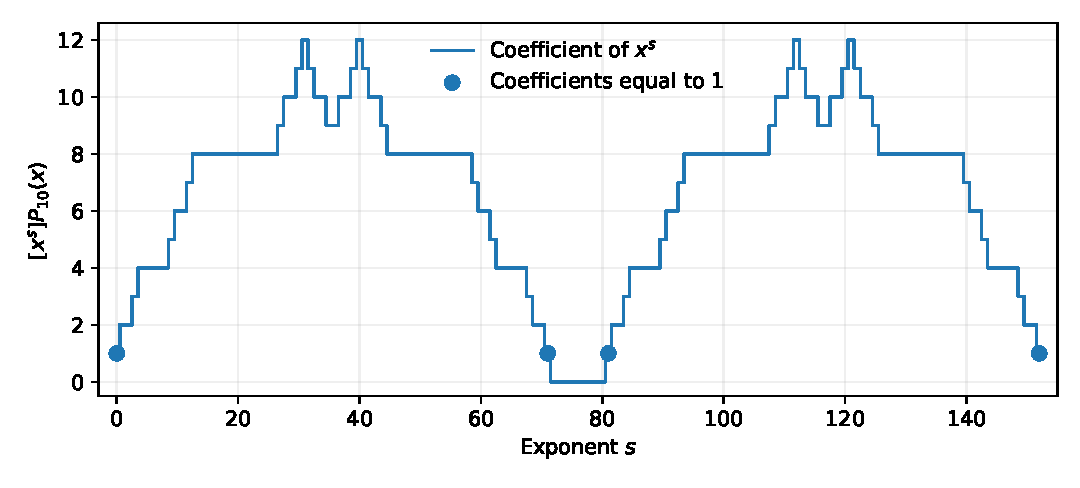
\includegraphics[width=0.97\linewidth]{figures/coefficient_profile.pdf}
\caption{The coefficients of $P_{10}=Q_{5,5}$. The four marked values occur
at the positions in \eqref{eq:examplelocations}. The maximum coefficient
is $12$; the sum of all coefficients is $2^{10}=1024$.}
\label{fig:profile}
\end{figure}

\section{An elementary obstruction to rationality}\label{sec:nonrational}

The exact count is a power of two. Its exponent grows at an irrational
average speed but changes only by zero or one at each step. Rational
generating functions cannot exhibit this particular combination.

\subsection{Rational recurrences modulo a prime}
A sequence is called \emph{eventually C-finite} when, from some index
onward, it satisfies a nontrivial linear recurrence with constant
coefficients; Definition~\ref{def:recurrences} states this and the
polynomial-coefficient analogue precisely, and both notions are used again
in Sections~\ref{sec:rigidity} and \ref{sec:boundary}. An ordinary
generating function over $\Q$ is rational if and only if its coefficients
are eventually C-finite over $\Q$: multiplying the series by its denominator gives
the recurrence, and summing an eventual recurrence gives a polynomial
numerator divided by a polynomial denominator.

There is no change in this conclusion if rationality is initially allowed
over $\C$ for a series with rational coefficients. For a fixed denominator
degree and a fixed numerator bound, the coefficient identities are linear
equations with rational entries in finitely many unknown denominator
coefficients, with the constant denominator coefficient normalized to one.
A finite subsystem spans all the augmented rows. If a complex solution
exists, rational Gaussian elimination gives a rational solution to that
subsystem and hence to all the identities. Thus the rational function can
be taken over $\Q$.

\begin{lemma}[Finite ratios and irrational exponent slope]\label{lem:finitefield}
Let $b\ge2$ and $C\ge1$ be integers. Suppose an integer sequence $(u_n)$
has, for all sufficiently large $n$, the form
\[
 u_n=C b^{e_n},\qquad e_n\in\Z_{\ge0},\qquad e_{n+1}-e_n\in\{0,1\}.
\]
If $\lim_{n\to\infty}e_n/n$ exists and is irrational, then
$\sum_{n\ge0}u_nz^n$ is not rational.
\end{lemma}
\begin{proof}
Suppose the generating function were rational. Then for some $d\ge1$
and rational constants $c_0,\ldots,c_{d-1}$,
\begin{equation}\label{eq:rationalrec}
 u_{n+d}=c_{d-1}u_{n+d-1}+\cdots+c_0u_n
\end{equation}
for every sufficiently large $n$. Choose a prime $p$ dividing neither
$Cb(b-1)$ nor any denominator of the $c_j$. Only finitely many primes
are excluded.

Reduce \eqref{eq:rationalrec} modulo $p$. The state vector
$(u_n,\ldots,u_{n+d-1})\bmod p$ belongs to the finite set $\F_p^d$ and
has a deterministic successor. Its forward orbit, and hence $u_n\bmod p$,
is eventually periodic. No invertibility of the transition is needed.

For large $n$, all $u_n\bmod p$ are nonzero. The quotient
$u_{n+1}/u_n\bmod p$ is therefore eventually periodic as well. Its actual
integer value is either $1$ or $b$, and these have distinct residues modulo
$p$. The periodic residue quotient thus uniquely determines the actual
quotient. Consequently $e_{n+1}-e_n$ is eventually periodic.

If its eventual period has length $L$ and contains $J$ ones, summing the
increments yields $e_n=(J/L)n+O(1)$. The limit $e_n/n$ must be the rational
number $J/L$, contrary to the hypothesis.
\end{proof}

\subsection{Applying the obstruction}
By its definition, $T(n)$ is nondecreasing. For $n\ge1$, if
$3^{T(n)}\ge2^{n+1}-1$, then
\[
 3^{T(n)+1}\ge3(2^{n+1}-1)\ge2^{n+2}-1.
\]
Therefore
\begin{equation}\label{eq:thresholdstep}
 T(n+1)-T(n)\in\{0,1\}\qquad(n\ge1).
\end{equation}
Moreover, the two adjacent powers bracketing the threshold give
\begin{equation}\label{eq:thresholdslope}
 T(n)=n\log_3 2+O(1).
\end{equation}
For $n\ge1$ put $e_n=n-T(n)+1$. Equations
\eqref{eq:diagonalcount}, \eqref{eq:thresholdstep}, and
\eqref{eq:thresholdslope} show that
\[
 a_n=2^{e_n},\qquad e_{n+1}-e_n\in\{0,1\},\qquad
 \frac{e_n}{n}\longrightarrow1-\log_3 2.
\]
The last limit is irrational. Indeed, a rational equality
$\log_3 2=p/q$ with positive integers $p,q$ would imply
$2^q=3^p$, contradicting unique prime factorization. Lemma~\ref{lem:finitefield}
proves that $A$ is not rational.

Finally, the even section of a rational series is rational. One way to see
this is to represent an eventual recurrence by a finite companion matrix:
sampling at even indices replaces the matrix by its square and again gives
a constant-coefficient recurrence, by the characteristic polynomial.
Equivalently,
\[
 \frac{F(t)+F(-t)}2=A(t^2),
\]
and an even rational function of $t$ is a rational function of $t^2$.
Thus rationality of $F$ would imply rationality of $A$, a contradiction.
This proves the negative answer to the universal rationality question.

This companion-matrix argument is exactly what the present section needs,
and no more: it handles the constant-coefficient case at $d=2$, $r=0$.
Lemma~\ref{lem:decimation} below proves the same closure property for all
arithmetic subsequences and for polynomial-coefficient recurrences, which is
what the non-D-finiteness of $F$ will require.

\begin{remark}[What the argument does not assume]
The irrationality of an exponential growth constant by itself would not
rule out rationality: coefficients of a rational function can have
irrational algebraic exponential growth. The proof instead uses an
irrational \emph{frequency of discrete exponent increments} and finite-state
arithmetic modulo a prime. It makes no algebraicity or transcendence claim
about $2^{1-\log_3 2}$.
\end{remark}

\section{Finite-quotient rigidity}\label{sec:rigidity}

The previous section is complete as an answer to the posed question. This
section gives a second, independent algebraic route to the same obstruction,
and the two are worth keeping side by side because they buy different things.

The modular argument of Section~\ref{sec:nonrational} is elementary and
entirely finite: it needs no invertibility of the transition, no field
extension, and no analysis. What it yields is nonrationality only, because
reducing a polynomial-coefficient recurrence modulo a prime does not produce
a finite-state system --- the coefficients then vary with $n$. The rigidity
theorem below works over $\C$, needs no prime and no reduction, and reaches
the strictly stronger conclusion that the counts are not P-recursive, hence
that their generating function is not D-finite. Neither argument subsumes
the other in difficulty or in hypotheses, so both are given in full.

This section also supplies no recurrence guessing from data and invokes no
theorem on zeros of recurrence sequences.

\begin{definition}[Recurrence classes]\label{def:recurrences}
A sequence $(u_n)$ of complex numbers is \emph{eventually C-finite} if there
exist constants $c_0,\ldots,c_s$, not all zero, with
\[
 \sum_{j=0}^s c_ju_{n+j}=0
 \qquad\hbox{for all sufficiently large }n.
\]
It is \emph{P-recursive} if the same holds with polynomials $p_j(n)\in\C[n]$,
not all zero, in place of the constants. Changing finitely many terms of a
sequence changes neither property, since both are required only eventually.
\end{definition}

\subsection{The rigidity theorem}
\begin{theorem}[Finite-quotient rigidity]\label{thm:rigidity}
Let $(u_n)$ be an eventually nonzero complex sequence whose adjacent
quotients $u_{n+1}/u_n$ lie in a fixed finite set. The following are
equivalent:
\begin{enumerate}[label=\textup{(\roman*)},leftmargin=2.4em]
\item $(u_n)$ is P-recursive;
\item $(u_n)$ is eventually C-finite;
\item the quotient sequence $\bigl(u_{n+1}/u_n\bigr)$ is eventually periodic.
\end{enumerate}
\end{theorem}
\begin{proof}
Discard an initial segment, so that every term used below is nonzero.
Implication (ii)$\Rightarrow$(i) is immediate from
Definition~\ref{def:recurrences}, since constants are polynomials. We prove
(i)$\Rightarrow$(ii), (ii)$\Rightarrow$(iii) and (iii)$\Rightarrow$(ii).

\smallskip\noindent\textbf{(i)$\Rightarrow$(ii).} Suppose
\begin{equation}\label{eq:Prec}
 \sum_{j=0}^sp_j(n)u_{n+j}=0
\end{equation}
for all large $n$, with some $p_j$ nonzero. The normalized vector
\[
 V_n=\left(1,\frac{u_{n+1}}{u_n},\ldots,\frac{u_{n+s}}{u_n}\right)
\]
takes only finitely many values: each coordinate is a product of at most $s$
members of the fixed finite quotient set. For each attainable vector
$v=(v_0,\ldots,v_s)$ form the polynomial
\[
 q_v(X)=\sum_{j=0}^sp_j(X)v_j.
\]
If $q_v$ is not identically zero it has only finitely many integer roots.
As there are finitely many such $v$, there is an $N_0$ exceeding every
nonnegative integer root of every nonzero $q_v$.

For $n\ge N_0$, dividing \eqref{eq:Prec} by $u_n$ says exactly
$q_{V_n}(n)=0$; by the choice of $N_0$ the polynomial $q_{V_n}$ must
therefore vanish identically. Let $d=\max_j\deg p_j$ and let $c_j$ be the
coefficient of $X^d$ in $p_j$, so that at least one $c_j$ is nonzero.
Comparing coefficients of $X^d$ in $q_{V_n}\equiv0$ gives
\[
 \sum_{j=0}^sc_j\frac{u_{n+j}}{u_n}=0,
 \qquad\hbox{hence}\qquad \sum_{j=0}^sc_ju_{n+j}=0
\]
for every $n\ge N_0$. This is a nontrivial constant-coefficient recurrence.

\smallskip\noindent\textbf{(ii)$\Rightarrow$(iii).} Choose an eventual
constant-coefficient recurrence whose largest index $s$ has $c_s\ne0$.
Necessarily $s\ge1$, since the terms are nonzero. If $s=1$ the quotient is
eventually the constant $-c_0/c_1$. For $s\ge2$ consider
\[
 W_n=\left(1,\frac{u_{n+1}}{u_n},\ldots,\frac{u_{n+s-1}}{u_n}\right),
\]
which again ranges over a finite set. The recurrence determines
$u_{n+s}/u_n$ from $W_n$, and dividing every shifted coordinate by the
nonzero entry $u_{n+1}/u_n$ then determines $W_{n+1}$ from $W_n$. So the
states follow a deterministic map on a finite set; their trajectory is
eventually periodic, and the second coordinate of $W_n$ is the adjacent
quotient.

\smallskip\noindent\textbf{(iii)$\Rightarrow$(ii).} If the quotients have
eventual period $p$, let $C$ be the product of the quotients over one
period. Then $u_{n+p}=Cu_n$ for all large $n$, a constant-coefficient
recurrence.
\end{proof}

\begin{corollary}[Irrational slope defeats P-recursiveness]\label{cor:slope}
Let $c\ge1$ be an integer, let $u_n>0$, and suppose that
$u_{n+1}/u_n\in\{1,c\}$ for all large $n$, with $c\ge2$. If
\[
 \lim_{n\to\infty}\frac{\log_cu_n}{n}
\]
exists and is irrational, then $(u_n)$ is not P-recursive, and therefore
$\sum_nu_nz^n$ is neither rational nor D-finite.
\end{corollary}
\begin{proof}
The quotients lie in the fixed finite set $\{1,c\}$. If they were eventually
periodic with period $p$ containing exactly $j$ occurrences of $c$, then
$\log_cu_n=(j/p)n+O(1)$ and the displayed limit would be the rational number
$j/p$. Theorem~\ref{thm:rigidity} therefore excludes P-recursiveness.
The final clause is the standard equivalence between D-finite series and
P-recursive coefficient sequences \cite[Theorem~1.5]{StanleyDFinite},
whose mechanism is recalled at the end of Section~\ref{sec:boundary}.
\end{proof}

Applied with $c=2$ to the binary--ternary counts, Corollary~\ref{cor:slope}
already gives more than Section~\ref{sec:nonrational} did. Equation
\eqref{eq:diagonalcount} together with \eqref{eq:thresholdstep} shows that
$a_{n+1}/a_n\in\{1,2\}$ for $n\ge1$, and \eqref{eq:thresholdslope} gives
\[
 \frac{\log_2a_n}{n}\longrightarrow1-\alpha=1-\log_32,
\]
which is irrational. Hence $(a_n)$ is not P-recursive. In
Section~\ref{sec:general} the same corollary is applied with $c=a$ to the
whole two-base family, using the quotient set $\{1,a\}$ supplied by
\eqref{eq:generalcount}.

\subsection{Passing to arithmetic subsequences}
The transfer from the even section to the full sequence must be proved, not
assumed; and for the D-finite conclusion it must be proved in the
polynomial-coefficient setting, which the companion-matrix argument of
Section~\ref{sec:nonrational} does not cover.

\begin{lemma}[Decimation]\label{lem:decimation}
Fix integers $d\ge1$ and $r\ge0$. If $(u_N)_{N\ge0}$ is P-recursive, then
$(u_{dn+r})_{n\ge0}$ is P-recursive. If $(u_N)$ is eventually C-finite, then
$(u_{dn+r})$ is eventually C-finite.
\end{lemma}
\begin{proof}
An order-zero recurrence $p_0(N)u_N=0$ with $p_0\ne0$ forces $u_N=0$ for all
large $N$, and the assertion is immediate. Otherwise take an order-$s$
recurrence with $s\ge1$. Away from the finitely many integer zeros of its
leading coefficient it can be solved for $u_{N+s}$ and written as
\[
 X_{N+1}=M(N)X_N,\qquad
 X_N=(u_N,u_{N+1},\ldots,u_{N+s-1})^{\mathsf T},
\]
with the entries of $M(N)$ rational functions of $N$. Composing $d$
consecutive steps and sampling at $N=dn+r$ gives a first-order system
\[
 Y_{n+1}=B(n)Y_n,\qquad Y_n=X_{dn+r},
\]
of the same dimension $s$, with entries rational in $n$. The first
coordinates of $Y_n,Y_{n+1},\ldots,Y_{n+s}$ are $s+1$ linear forms in the
$s$ coordinates of $Y_n$, with coefficients in $\C(n)$; any $s+1$ linear
forms in $s$ variables are linearly dependent over that field. Clearing
denominators turns such a dependence into a nonzero
polynomial-coefficient recurrence for $(u_{dn+r})$. If the original
coefficients are constant, then $M$ is constant, $B=M^d$ is constant, and
the same argument produces constant coefficients.
\end{proof}

Consequently $(\nu(N))$ is not P-recursive either: its even subsequence
$(a_n)$ is not, and Lemma~\ref{lem:decimation} with $d=2$, $r=0$ would
otherwise make it so. This completes the second algebraic route, and it
establishes non-P-recursiveness of both sequences --- a conclusion that
Section~\ref{sec:nonrational} does not reach.

\section{The floor formula and the odd indices}\label{sec:floor}

\subsection{Removing the near-integer ambiguity}
The threshold \eqref{eq:threshold} involves $2^{n+1}-1$, not $2^{n+1}$.
The difference is important for the initial terms and must not be silently
dropped.

\begin{proposition}[Exact floor expression]\label{prop:floor}
For $n\ge2$,
\begin{equation}\label{eq:Tfloor}
 T(n)=\ceil{(n+1)\alpha}=\floor{(n+1)\alpha}+1,
 \qquad \alpha=\log_3 2.
\end{equation}
Consequently \eqref{eq:mainformula} holds for every $n\ge0$.
\end{proposition}
\begin{proof}
Let $M=\ceil{(n+1)\alpha}$ be the least integer such that
$3^M\ge2^{n+1}$. The number $(n+1)\alpha$ is irrational, so the inequality
is strict and the ceiling is one more than the floor.
Since the smaller threshold in \eqref{eq:threshold} is $2^{n+1}-1$,
we have $T(n)\le M$. If $T(n)<M$, an integer power of three is at least
$2^{n+1}-1$ but smaller than $2^{n+1}$. It must equal $2^{n+1}-1$.
For $n\ge2$, the latter is $7$ modulo $8$, whereas a power of three is
$1$ or $3$ modulo $8$. This is impossible.

Substitute \eqref{eq:Tfloor} into \eqref{eq:diagonalcount}. At $n=0$,
$2^{0-\lfloor\alpha\rfloor}=1=a_0$. At $n=1$,
$2^{1-\lfloor2\alpha\rfloor}=1$ while $a_1=2$, producing exactly the
correction $\ind{n=1}$.
\end{proof}

For $n\ge2$ the logarithmic exponent increments can also be written as
\begin{equation}\label{eq:rotationincrements}
 \log_2\frac{a_{n+1}}{a_n}
 =1-\bigl(\floor{(n+2)\alpha}-\floor{(n+1)\alpha}\bigr).
\end{equation}
This is a binary sequence driven by an irrational rotation. Its long-run
frequency of ones is $1-\alpha$, either by telescoping the floors or by
the equidistribution argument in the next section. In particular, the
proportion of indices at which $a_n$ doubles tends to $1-\alpha$.

\subsection{The doubling word}\label{sec:doublingword}
It is worth making the coding in \eqref{eq:rotationincrements} completely
explicit, because it is the exact point at which an irrational number enters
a purely combinatorial sequence. Write $u_n=\fracpart{(n+1)\alpha}$, as in
\eqref{eq:constants} below. For $n\ge2$ the value \eqref{eq:rotationincrements}
equals $1$ --- that is, $a_{n+1}=2a_n$ --- precisely when
$\floor{(n+2)\alpha}=\floor{(n+1)\alpha}$, and hence precisely when
\begin{equation}\label{eq:sturmian}
 u_n<1-\alpha.
\end{equation}
Otherwise $a_{n+1}=a_n$. The doubling word
$(\ind{u_n<1-\alpha})_{n\ge2}$ is therefore a Sturmian coding of the
rotation by $\alpha$, and by Lemma~\ref{lem:rotation} its limiting
proportion of ones is the length $1-\alpha$ of the coding interval.

This yields the obstruction of Section~\ref{sec:rigidity} in one line:
no eventually periodic binary word has an irrational proportion of ones,
because the proportion of an eventually periodic word is the number of ones
in one period divided by the period length. So the doubling word is not
eventually periodic, so by Theorem~\ref{thm:rigidity} the sequence $(a_n)$
--- whose adjacent quotients are exactly the letters of that word, read as
$1$ and $2$ --- is not P-recursive.

\subsection{The entire product-length sequence}
The rectangular formula also determines the odd indices without a new
counting argument.

\begin{proposition}[Even--odd identity]\label{prop:odd}
For every $n\ge0$,
\begin{equation}\label{eq:odd}
 b_n=\frac{a_{n+1}}2+\ind{0\le n\le3}.
\end{equation}
Thus
\begin{equation}\label{eq:fullrelation}
 F(t)=\frac{(2t+1)A(t^2)-1}{2t}+t+t^3+t^5+t^7,
\end{equation}
where the apparent singularity at $t=0$ is removable.
\end{proposition}
\begin{proof}
For $n\ge1$, Theorem~\ref{thm:rectangle} gives
$b_n=2^{1+\max(0,n-T(n+1))}$, while
$a_{n+1}/2=2^{n+1-T(n+1)}$.
The bound $T(n+1)\le n+1$ shows that these agree unless
$T(n+1)=n+1$, in which case their values are $2$ and $1$.
Directly, $T(2)=2$, $T(3)=3$, and $T(4)=4$.
For $n\ge4$ the inequality $3^n\ge2^{n+2}-1$ follows from its case
$n=4$ by induction; hence $T(n+1)\le n$. At $n=0$ the required identity
is $b_0=2=a_1/2+1$.

Writing $B(z)=\sum_{n\ge0}b_nz^n$, summation gives
\[
 B(z)=\frac{A(z)-1}{2z}+1+z+z^2+z^3.
\]
Substitute this into $F(t)=A(t^2)+tB(t^2)$ to obtain
\eqref{eq:fullrelation}.
\end{proof}

Proposition~\ref{prop:odd} is the $(a,q)=(2,3)$ instance of a general
even--odd identity; Proposition~\ref{prop:generalparity} and
Corollary~\ref{cor:binaryparity} in Section~\ref{sec:general} give the
statement for every pair of bases, with the exceptional index set computed
explicitly for $a=2$. The correction $\ind{0\le n\le3}$ here is not an
artefact of small numbers but the complete list of indices at which the
threshold saturates; for $q\ge5$ the analogous list is empty.

The initial values, indexed by the actual number of factors, are
\begin{equation}\label{eq:fullterms}
\begin{split}
 (\nu(N))_{N=0}^{22}={}&(1,2,2,2,2,2,2,2,2,2,4,2,\\
                     &\hphantom{(}4,2,4,4,8,4,8,8,16,8,16).
\end{split}
\end{equation}
The drops at odd indices are real; adding a factor can turn many coefficients
that were one into larger coefficients. The even subsequence is monotone,
but the full coefficient-one sequence need not be.

\section{Asymptotics with persistent oscillation}\label{sec:asymptotics}

Set
\begin{equation}\label{eq:constants}
 \lambda=2^{1-\alpha},\qquad R=\lambda^{-1},\qquad
 h(u)=2^{u-\alpha}\quad(0\le u<1),\qquad
 u_n=\fracpart{(n+1)\alpha}.
\end{equation}
Numerically,
\[
 \alpha\approx0.630929753571,\quad
 \lambda\approx1.291520234330,\quad
 R\approx0.774281326315.
\]
These decimal approximations play no role in the exact computations or
proofs. Proposition~\ref{prop:floor} gives the exact representation
\begin{equation}\label{eq:profile}
 a_n=\lambda^n h(u_n)+\ind{n=1}.
\end{equation}
Thus the relative fluctuations do not shrink with $n$; they are the values
of a fixed function sampled along an irrational rotation.

\subsection{The equidistribution input}
We use the following elementary consequence of the geometric-sum formula.

\begin{lemma}[Irrational rotation averages]\label{lem:rotation}
If $\beta$ is irrational and $f$ is Riemann integrable on $[0,1]$, with
its values interpreted periodically, then for every real $\gamma$,
\begin{equation}\label{eq:equidistribution}
 \lim_{M\to\infty}\frac1M\sum_{n=0}^{M-1}
 f(\fracpart{n\beta+\gamma})=\int_0^1f(u)\,du.
\end{equation}
\end{lemma}
\begin{proof}
For each nonzero integer $j$,
\[
 \frac1M\sum_{n=0}^{M-1}e^{2\pi i j(n\beta+\gamma)}
 =\frac{e^{2\pi i j\gamma}}{M}
   \frac{1-e^{2\pi i jM\beta}}{1-e^{2\pi i j\beta}}
 \longrightarrow0.
\]
For $j=0$ the average is $1$. Therefore \eqref{eq:equidistribution} holds
for trigonometric polynomials. Uniform approximation by trigonometric
polynomials extends it to continuous periodic functions.
Continuous upper and lower approximations to an interval indicator then
give its average as the interval length: the approximations can differ only
in arbitrarily short neighborhoods of the endpoints. Finite step functions
follow. Finally, upper and lower Riemann sums approximate every real Riemann
integrable $f$ with arbitrarily small integral gap. Apply the same argument
to the real and imaginary parts for complex-valued $f$.
\end{proof}

\begin{proposition}[Growth and fluctuation law]\label{prop:growth}
The sequence $a_n$ satisfies
\begin{equation}\label{eq:growthroot}
 \lim_{n\to\infty}a_n^{1/n}=\lambda,
 \qquad a_n=\Theta(\lambda^n).
\end{equation}
The set of limit points of $a_n/\lambda^n$ is the whole interval
\begin{equation}\label{eq:limitinterval}
 [2^{-\alpha},\ 2^{1-\alpha}].
\end{equation}
In particular there is no constant $C$ for which $a_n\sim C\lambda^n$.
Its normalized Ces\`aro mean does exist:
\begin{equation}\label{eq:cesaromean}
 \lim_{M\to\infty}\frac1M\sum_{n=0}^{M-1}\frac{a_n}{\lambda^n}
 =\frac{2^{-\alpha}}{\log 2}.
\end{equation}
The full sequence has root growth
$\lim_{N\to\infty}\nu(N)^{1/N}=\sqrt\lambda$.
\end{proposition}
\begin{proof}
Outside the single corrected index, \eqref{eq:profile} lies between the
two fixed positive bounds $2^{-\alpha}\lambda^n$ and
$2^{1-\alpha}\lambda^n$. This proves \eqref{eq:growthroot}.
Lemma~\ref{lem:rotation} implies that the fractional parts $u_n$ visit
every subinterval of $[0,1)$ infinitely often. The strictly increasing
function $h$ therefore gives every interior point of
\eqref{eq:limitinterval} as a subsequential limit; approaching $0$ and $1$
gives the endpoints. No other limits are possible. Equation
\eqref{eq:cesaromean} follows by integrating $h$, and the finite exceptional
term vanishes in the average. Finally, \eqref{eq:odd} gives the same
root growth on both parities of $\nu(N)$.
\end{proof}

\subsection{The exact law of the fluctuations}
Proposition~\ref{prop:growth} identifies the closure of the set of
fluctuation values and their mean. Equidistribution in fact delivers the
entire limiting distribution, not merely its support and its first moment.

\begin{proposition}[Limiting distribution of the normalized counts]
\label{prop:distribution}
For every $y$ with $2^{-\alpha}\le y\le2^{1-\alpha}$,
\begin{equation}\label{eq:distribution}
 \lim_{N\to\infty}\frac1N\,
 \#\left\{2\le n<N:\ \frac{a_n}{\lambda^n}\le y\right\}
 =\alpha+\log_2y.
\end{equation}
The limiting law is supported on $[2^{-\alpha},2^{1-\alpha}]$ with density
$1/(y\log2)$ there, and its mean is the Ces\`aro value
$2^{-\alpha}/\log2$ of \eqref{eq:cesaromean}.
\end{proposition}
\begin{proof}
For $n\ge2$, \eqref{eq:profile} gives $a_n/\lambda^n=h(u_n)=2^{u_n-\alpha}$
with $u_n=\fracpart{(n+1)\alpha}$. Since $h$ is strictly increasing, the
event $h(u_n)\le y$ is the event $u_n\le\alpha+\log_2y$, and the right-hand
side lies in $[0,1]$ exactly on the stated range of $y$. Apply
Lemma~\ref{lem:rotation} to the indicator of $[0,\alpha+\log_2y]$, which is
Riemann integrable, with $\beta=\alpha$ and $\gamma=\alpha$. The density is
obtained by differentiating $\alpha+\log_2y$, and
$\int_{2^{-\alpha}}^{2^{1-\alpha}}y\cdot\frac{dy}{y\log2}
 =\int_0^12^{u-\alpha}\,du=2^{-\alpha}/\log2$.
\end{proof}

\begin{remark}[Two normalizations of the same law]\label{rem:normalization}
It is equally natural to divide by $\lambda^{n+1}$ rather than $\lambda^n$.
Because $\lambda=2^{1-\alpha}$ and, by irrationality,
$\fracpart{(n+1)(1-\alpha)}=1-\fracpart{(n+1)\alpha}$, the two normalized
quantities are related by
\begin{equation}\label{eq:normalizationshift}
 \frac{a_n}{\lambda^{n+1}}=\frac1\lambda\cdot\frac{a_n}{\lambda^n}
 =2^{\,u_n-1}=2^{-\fracpart{(n+1)(1-\alpha)}}\qquad(n\ge2).
\end{equation}
In that normalization the support is $[1/2,1]$, the distribution function
\eqref{eq:distribution} reads $1+\log_2y$, and the mean becomes
$\int_0^12^{-x}\,dx=1/(2\log2)$. The two means differ by exactly the factor
$\lambda$, as \eqref{eq:normalizationshift} requires; neither is a competing
claim about the same quantity. All statements in this report use the
$\lambda^n$ normalization of \eqref{eq:constants}.
\end{remark}

\begin{figure}[htbp]
\centering
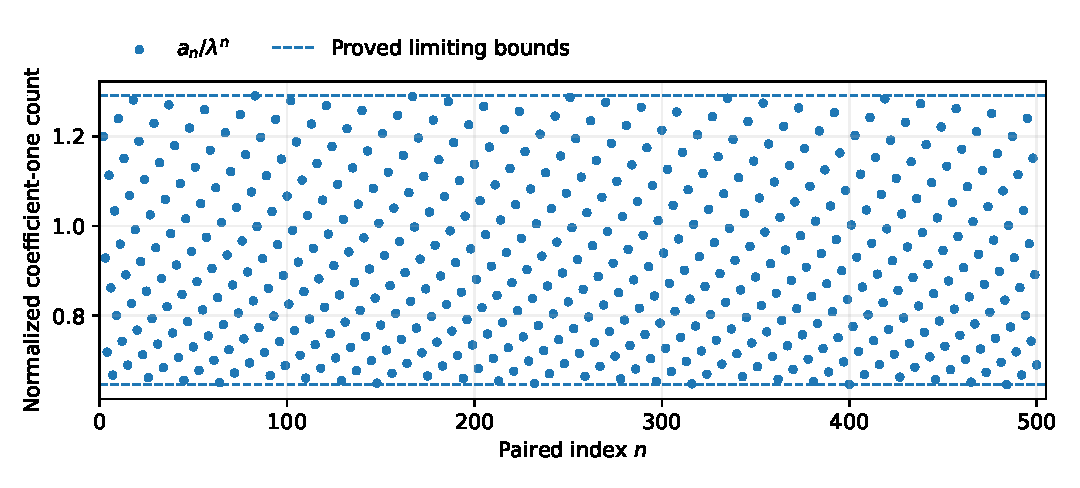
\includegraphics[width=0.97\linewidth]{figures/normalized_counts.pdf}
\caption{The normalized counts $a_n/\lambda^n$ for $2\le n\le500$.
The dashed lines are the limiting bounds in \eqref{eq:limitinterval}.
The nonvanishing oscillation is proved by irrational rotation, not inferred
from this plot. Floating-point arithmetic is used only to draw the figure.}
\label{fig:oscillation}
\end{figure}

\section{Dense singularities and a natural boundary}\label{sec:boundary}

The fluctuation law does more than prevent a constant leading asymptotic.
Every Fourier mode of the profile $h$ is nonzero. Each mode produces a
boundary singularity, and the corresponding points are dense on the circle
of convergence.

\subsection{A precise Abelian lemma}
\begin{lemma}[Ces\`aro means imply radial limits]\label{lem:abel}
Let $(c_n)$ be a bounded complex sequence. If
$M^{-1}\sum_{n=0}^{M-1}c_n\to c$, then
\begin{equation}\label{eq:abel}
 \lim_{\rho\uparrow1}(1-\rho)\sum_{n\ge0}c_n\rho^n=c.
\end{equation}
\end{lemma}
\begin{proof}
Put $S_N=\sum_{n=0}^Nc_n$. Absolute convergence for $0<\rho<1$ gives
\[
 \sum_{n\ge0}c_n\rho^n=(1-\rho)\sum_{N\ge0}S_N\rho^N.
\]
The hypothesis is $S_N=(N+1)c+o(N+1)$. Since
$\sum_{N\ge0}(N+1)\rho^N=(1-\rho)^{-2}$, the principal term contributes
$c$ after multiplying by $1-\rho$. For the error, fix $\varepsilon>0$ and
choose $N_0$ so that its absolute value is at most
$\varepsilon(N+1)$ for $N\ge N_0$. The tail contributes at most
$\varepsilon$, and the finitely many initial terms tend to zero. This
proves \eqref{eq:abel}.
\end{proof}

\subsection{Nonzero radial amplitudes at a dense set}
\begin{theorem}[Explicit dense boundary singularities]\label{thm:boundary}
For each $k\in\Z$, put $\omega_k=e^{-2\pi i k\alpha}$. Then
\begin{equation}\label{eq:radial}
 \lim_{\rho\uparrow1}(1-\rho)A(R\rho\omega_k)
 =\frac{2^{-\alpha}e^{2\pi i k\alpha}}{\log 2-2\pi i k}\ne0.
\end{equation}
The circle $|z|=R$ is a natural boundary of $A$.
\end{theorem}
\begin{proof}
Equation~\eqref{eq:growthroot} shows that the radius of convergence is
exactly $R$. Ignore the single correction at $n=1$ for the moment.
At $z=R\rho\omega_k$, formula \eqref{eq:profile} makes the summand
$h(u_n)\omega_k^n\rho^n$. Since
\[
 \omega_k^n=e^{2\pi i k\alpha}e^{-2\pi i k u_n},
\]
Lemma~\ref{lem:rotation}, applied to the Riemann integrable function
$h(u)e^{-2\pi i k u}$, gives the Ces\`aro mean
\begin{align*}
 \lim_{M\to\infty}\frac1M\sum_{n=0}^{M-1}h(u_n)\omega_k^n
 &=e^{2\pi i k\alpha}\int_0^1 2^{u-\alpha}e^{-2\pi i k u}\,du\\
 &=\frac{2^{-\alpha}e^{2\pi i k\alpha}}{\log2-2\pi i k}.
\end{align*}
In the integral, $e^{\log2-2\pi i k}-1=1$. The resulting value is nonzero
for every integer $k$. Lemma~\ref{lem:abel} proves \eqref{eq:radial}.
The omitted correction contributes $(1-\rho)R\rho\omega_k$, which tends
to zero.

If $A$ admitted a holomorphic extension across the point $R\omega_k$, it
would remain bounded along the inward radial segment near that point.
Equation~\eqref{eq:radial} contradicts this. Thus every $R\omega_k$ is a
singular point. Irrationality of $\alpha$ makes the set of $\omega_k$ dense
on the unit circle. An extension across any other point of $|z|=R$ would
be defined in an open neighborhood containing some $R\omega_k$, again a
contradiction. Hence no point on the circle admits analytic continuation
through the circle.
\end{proof}

The limit \eqref{eq:radial} describes a radial blowup. It does \emph{not}
assert that these are isolated poles or provide residues of a meromorphic
continuation: the singularities are dense, and no such neighborhood of
continuation is available.

\subsection{A second proof, from a general irrational-floor theorem}
\label{sec:floorboundary}
Theorem~\ref{thm:boundary} is a direct computation on the actual coefficient
profile $h$ of \eqref{eq:constants}. The same conclusion follows from a
general principle in which the profile is first normalized to the clean
exponential $q^{-x}$, at the cost of an extra transfer step. Both proofs are
kept: the first stays inside the concrete problem and needs no auxiliary
series, while the second proves considerably more --- it covers every
irrational exponent and every base at once, so it settles the whole family
of Section~\ref{sec:general} without a new computation.

Let $0<\theta<1$ be irrational and let $q>1$ be real. Define
\begin{equation}\label{eq:Phidef}
 \Phi_{\theta,q}(w)=\sum_{n\ge0}q^{\floor{n\theta}}w^n,
 \qquad \Lambda=q^\theta,
\end{equation}
and its normalization
\begin{equation}\label{eq:Psidef}
 \Psi(w)=\Phi_{\theta,q}(w/\Lambda)=\sum_{n\ge0}q^{-\fracpart{n\theta}}w^n .
\end{equation}
The coefficients of $\Psi$ lie between $q^{-1}$ and $1$, so its radius of
convergence is exactly $1$.

\begin{theorem}[Natural boundary for an irrational-floor series]
\label{thm:floorboundary}
For every irrational $\theta\in(0,1)$ and every $q>1$, the circle
$|w|=q^{-\theta}$ is a natural boundary of $\Phi_{\theta,q}$. More precisely,
for each $k\in\Z$, with $\zeta_k=e^{-2\pi ik\theta}$,
\begin{equation}\label{eq:radialabstract}
 \lim_{\rho\uparrow1}(1-\rho)\Psi(\rho\zeta_k)
 =\frac{1-q^{-1}}{\log q+2\pi ik}\ne0,
\end{equation}
and the unit circle is a natural boundary of $\Psi$.
\end{theorem}
\begin{proof}
On $0\le x<1$ put $f(x)=q^{-x}$ and extend $f$ periodically. For a fixed
integer $k$ the function $f(x)e^{-2\pi ikx}$ is bounded and Riemann
integrable. Since
$\zeta_k^{\,n}=e^{-2\pi ikn\theta}=e^{-2\pi ik\fracpart{n\theta}}$,
the $n$th coefficient of $\Psi$ evaluated along the ray through $\zeta_k$ is
$f(\fracpart{n\theta})e^{-2\pi ik\fracpart{n\theta}}$. Lemma~\ref{lem:rotation}
with $\beta=\theta$ and $\gamma=0$ therefore gives the Ces\`aro mean
\[
 \lim_{N\to\infty}\frac1N\sum_{n=0}^{N-1}q^{-\fracpart{n\theta}}\zeta_k^{\,n}
 =\int_0^1q^{-x}e^{-2\pi ikx}\,dx
 =\frac{1-q^{-1}}{\log q+2\pi ik},
\]
using $e^{-\log q-2\pi ik}=q^{-1}$. The value is nonzero for every $k$
because $q>1$. Lemma~\ref{lem:abel}, applied to the bounded sequence
$q^{-\fracpart{n\theta}}\zeta_k^{\,n}$, converts this into
\eqref{eq:radialabstract}.

If $\Psi$ extended holomorphically through $\zeta_k$ it would be bounded on
a short inward radial segment ending there, forcing the limit in
\eqref{eq:radialabstract} to vanish. So every $\zeta_k$ is a singular point
of $\Psi$. Irrationality of $\theta$ makes $\{\zeta_k:k\in\Z\}$ dense on the
unit circle, and an extension through any boundary point would be defined on
an open arc, which contains some $\zeta_k$. Hence the unit circle is a
natural boundary of $\Psi$, and the substitution $w\mapsto w/\Lambda$
transports this to the circle $|w|=\Lambda^{-1}=q^{-\theta}$ for
$\Phi_{\theta,q}$.
\end{proof}

\begin{remark}[Averages, not formal Fourier series]\label{rem:fourier}
The proof evaluates explicit Ces\`aro averages of the sequence
$q^{-\fracpart{n\theta}}\zeta_k^{\,n}$. It does not expand the discontinuous
periodic profile in a Fourier series and then evaluate that series
termwise. The distinction matters: the periodic extension of $q^{-x}$ has a
jump at the integers, and a formal Fourier expansion would need a separate
convergence argument exactly there. Lemma~\ref{lem:rotation} is stated for
Riemann integrable $f$ precisely so that no such argument is needed. This
complements, and does not repeat, the caution after \eqref{eq:radial}: that
remark concerns what the radial limit does not say about poles or residues,
whereas this one concerns how the limit is computed.
\end{remark}

\subsubsection*{Transfer to the count series}
Applying Theorem~\ref{thm:floorboundary} to the counts requires an exact
bridge, because the floor in \eqref{eq:mainformula} is written with $\alpha$
and the theorem is stated with the complementary exponent. The two agree:
since $(n+1)\alpha$ is irrational,
\begin{equation}\label{eq:floorcomplement}
 \floor{(n+1)(1-\alpha)}
 =(n+1)-\ceil{(n+1)\alpha}
 =n-\floor{(n+1)\alpha}\qquad(n\ge0),
\end{equation}
so the exponent $n-\floor{(n+1)\alpha}$ of \eqref{eq:mainformula} is the
floor $\floor{(n+1)\theta}$ of Theorem~\ref{thm:floorboundary} at
$\theta=1-\alpha$ and $q=2$. This identity is stated once here and used
without further comment; the two closed forms are the same closed form.

Write $\Phi=\Phi_{1-\alpha,2}$, so that $\Lambda=2^{1-\alpha}=\lambda$ and
the radius of convergence of $\Phi$ is $\lambda^{-1}=R$. Then
\begin{equation}\label{eq:transfer}
 A(z)=\frac{\Phi(z)-1}{z}+z .
\end{equation}
Indeed, $[z^n]\bigl(\Phi(z)-1\bigr)/z=2^{\floor{(n+1)(1-\alpha)}}
=2^{\,n-\floor{(n+1)\alpha}}$ by \eqref{eq:floorcomplement}, which is $a_n$
for every $n$ except $n=1$, where it is $1$ instead of $2$; the added $z$
corrects exactly that term, in agreement with the $\ind{n=1}$ of
\eqref{eq:mainformula}. Equation \eqref{eq:transfer} is equivalent to
$\Phi(z)=z\bigl(A(z)-z\bigr)+1$, so each of $A$ and $\Phi$ is an analytic
function of the other on any open set avoiding $z=0$. A holomorphic
extension of $A$ through a point of $|z|=R$ would therefore extend $\Phi$
through the same point, which Theorem~\ref{thm:floorboundary} forbids.
This reproves the last assertion of Theorem~\ref{thm:boundary} from a
statement that makes no reference to the enumeration.

\begin{remark}[Reconciling the two radial constants]\label{rem:reconcile}
Theorem~\ref{thm:boundary} and Theorem~\ref{thm:floorboundary} display
constants that look different --- the sign of $2\pi ik$ is opposite and one
carries a phase $e^{2\pi ik\alpha}$ --- but they are the same statement in
two index conventions, and \eqref{eq:transfer} converts one into the other
exactly. First, the two families of boundary directions coincide with
reversed index: with $\theta=1-\alpha$,
\[
 \zeta_k=e^{-2\pi ik(1-\alpha)}=e^{2\pi ik\alpha}=\omega_{-k},
 \qquad\hbox{equivalently}\qquad \omega_k=\zeta_{-k}.
\]
So \eqref{eq:radialabstract} at $q=2$, read at the direction $\omega_k$,
gives $\lim(1-\rho)\Psi(\rho\omega_k)=\tfrac12/(\log2-2\pi ik)$. Second,
multiplying \eqref{eq:transfer} by $1-\rho$ at $z=R\rho\omega_k$ and letting
$\rho\uparrow1$ kills the terms $-(1-\rho)/z$ and $(1-\rho)z$ and leaves
\[
 \lim_{\rho\uparrow1}(1-\rho)A(R\rho\omega_k)
 =\frac1{R\omega_k}\lim_{\rho\uparrow1}(1-\rho)\Psi(\rho\omega_k)
 =\frac{e^{2\pi ik\alpha}}{2^{\alpha-1}}\cdot\frac{1/2}{\log2-2\pi ik},
\]
using $\Phi(R\rho\omega_k)=\Psi(\rho\omega_k)$ and $R=2^{\alpha-1}$. As
$\tfrac12\cdot2^{1-\alpha}=2^{-\alpha}$, the right-hand side is
$2^{-\alpha}e^{2\pi ik\alpha}/(\log2-2\pi ik)$, which is exactly
\eqref{eq:radial}. The apparent discrepancy is entirely the index reversal
$k\mapsto-k$ together with the factor $1/(R\omega_k)$ contributed by the
transfer.
\end{remark}

\subsection{The full generating function and recurrence consequences}
\begin{corollary}\label{cor:fullboundary}
The circle $|t|=\sqrt R$ is a natural boundary of $F$.
\end{corollary}
\begin{proof}
Equation~\eqref{eq:fullrelation} makes $F$ holomorphic for
$|t|<\sqrt R$, with a removable singularity at zero. Suppose it extended
through some point $t_0$ on the boundary. Since $t_0\ne0$, the map
$t\mapsto t^2$ has a local analytic inverse near $t_0$. Also
$2t_0+1\ne0$: the only zero is $-1/2$, whereas
$\sqrt R>1/\sqrt2>1/2$. Solving \eqref{eq:fullrelation} for $A(t^2)$ would
therefore provide an analytic extension of $A$ through $t_0^2$, contrary
to Theorem~\ref{thm:boundary}.
\end{proof}

A power series $H(z)$ is D-finite if it satisfies a nonzero homogeneous
linear differential equation
\begin{equation}\label{eq:dfinite}
 p_d(z)H^{(d)}(z)+\cdots+p_0(z)H(z)=0,
 \qquad p_j(z)\in\C[z],\quad p_d\ne0.
\end{equation}
This is the standard terminology developed in \cite{StanleyDFinite}, where
the equivalence between D-finite series and P-recursive coefficient
sequences is \cite[Theorem~1.5]{StanleyDFinite}; the direct mechanism is
recalled below so that nothing here depends on an unstated import.
Away from the finitely many zeros of $p_d$, a linear differential equation
has analytic coefficients after division by $p_d$; its local solutions
continue along paths avoiding those zeros. An analytic germ satisfying
\eqref{eq:dfinite} cannot therefore have a natural boundary on a finite
circle.

Likewise, an algebraic germ has only finitely many possible finite
singularities. For an irreducible polynomial equation $p(z,H)=0$ of positive degree in $H$, exclude
the zeros of its leading coefficient in $H$ and of its discriminant in
$H$; the implicit-function theorem gives local analytic branches at the
remaining points. This also contradicts a natural boundary.

Finally, a sequence $(u_n)$ is P-recursive if it satisfies an eventual
nonzero linear recurrence with polynomial coefficients in $n$. Such a
recurrence implies a D-finite generating function. To recall the direct
mechanism, let $\theta=z\,d/dz$. Then $\theta(z^n)=nz^n$, so sums of
$p_j(n)u_{n+j}z^n$ can be written as differential operators in $\theta$
applied to $H(z)=\sum u_nz^n$, up to finitely many initial terms.
After clearing powers of $z$, the recurrence becomes a nonzero linear
differential equation with a polynomial right-hand side. Differentiating
sufficiently many times makes that right-hand side zero. These observations
and the two natural-boundary results prove all remaining conclusions of
Theorem~\ref{thm:main}.

\section{A complete classification for two bases}\label{sec:general}

The counterexample is part of a family in which the rationality question
can be answered exactly. Fix integers $2\le a<q$ and define the digit
polynomial
\begin{equation}\label{eq:digitpoly}
 D_a(y)=1+y+\cdots+y^{a-1}.
\end{equation}
Use the interleaved exponents
\begin{equation}\label{eq:generalexponents}
 G_{2j+1}=a^j,\qquad G_{2j+2}=q^j,
\end{equation}
and the products $\prod_{i=1}^N D_a(x^{G_i})$. This is precisely
\eqref{eq:stanleyproduct} with fixed $r=a-1$. The exponent generating
function is $t/(1-at^2)+t^2/(1-qt^2)$, and $G_N\to\infty$.
Let $v_{a,q}(N)$ count the coefficients equal to one and put
\begin{equation}\label{eq:generalseries}
 F_{a,q}(t)=\sum_{N\ge0}v_{a,q}(N)t^N,
 \qquad
 A_{a,q}(z)=\sum_{n\ge0}v_{a,q}(2n)z^n,
\end{equation}
so that $A_{a,q}$ is the even section of $F_{a,q}$, exactly as $A$ is of
$F$ in \eqref{eq:ABF}. Two integers $a,q>1$ are \emph{multiplicatively
dependent} when $q^u=a^v$ for some positive integers $u,v$; equivalently,
$\log_q a$ is rational.

\begin{theorem}[Two-base classification]\label{thm:classification}
For every pair of integers $2\le a<q$, the following five statements are
equivalent:
\begin{enumerate}[label=\textup{(\roman*)},leftmargin=2.4em]
\item $a$ and $q$ are multiplicatively dependent;
\item $A_{a,q}(z)$ is rational;
\item $A_{a,q}(z)$ is D-finite;
\item $F_{a,q}(t)$ is rational;
\item $F_{a,q}(t)$ is D-finite.
\end{enumerate}
In particular
\begin{equation}\label{eq:classification}
 F_{a,q}(t)\text{ is rational}
 \quad\Longleftrightarrow\quad
 a\text{ and }q\text{ are multiplicatively dependent},
\end{equation}
and when the bases are independent neither series is D-finite and neither
count sequence is P-recursive.
When $q^u=a^v$ with $u,v\ge1$, necessarily $v>u$, and
\begin{equation}\label{eq:eventualdependent}
 v_{a,q}(N+2v)=a^{v-u}v_{a,q}(N)
\end{equation}
for every sufficiently large $N$. In particular the reduced denominator
of $F_{a,q}(t)$ divides $1-a^{v-u}t^{2v}$.
\end{theorem}

For $a=2$ the dependence condition takes a familiar shape: $2$ and $q$ are
multiplicatively dependent exactly when $q$ is a power of two, since
$q^u=2^v$ forces every prime divisor of $q$ to be $2$. So the statement
``$q$ is a power of two'' that governs the binomial subfamily
$D_2(y)=1+y$ is precisely the $a=2$ instance of multiplicative dependence,
and Theorem~\ref{thm:classification} contains it.

The proof occupies the rest of this section and closes the cycle
\[
 \hbox{(i)}\Rightarrow\hbox{(ii)}\Rightarrow\hbox{(iii)}
 \Rightarrow\hbox{(i)},
 \qquad
 \hbox{(i)}\Rightarrow\hbox{(iv)}\Rightarrow\hbox{(v)}
 \Rightarrow\hbox{(iii)}.
\]
Subsection~\ref{sec:genrect} proves the enumerative formula that everything
rests on. Subsection~\ref{sec:genindep} proves (iii)$\Rightarrow$(i) and
(v)$\Rightarrow$(iii), both in contrapositive form and both using
Section~\ref{sec:rigidity}; the second also uses
Lemma~\ref{lem:decimation}. Subsection~\ref{sec:gendep} proves
(i)$\Rightarrow$(ii) and (i)$\Rightarrow$(iv). The implications
(ii)$\Rightarrow$(iii) and (iv)$\Rightarrow$(v) are immediate, because a
rational function satisfies a first-order linear differential equation with
polynomial coefficients. Subsection~\ref{sec:genparity} is not needed for
the equivalence itself; it makes the passage between $A_{a,q}$ and
$F_{a,q}$ explicit, and generalizes Proposition~\ref{prop:odd}.

\subsection{Exact counts for a general rectangle}\label{sec:genrect}
Write
\begin{equation}\label{eq:generalrectangle}
 Q^{a,q}_{m,n}(x)=
 \prod_{j=0}^{m-1}D_a(x^{a^j})
 \prod_{j=0}^{n-1}D_a(x^{q^j}),
\end{equation}
and let $U_{a,q}(m,n)$ be its number of coefficients equal to one.
The first product is $1+x+\cdots+x^{a^m-1}$. The second is supported,
with coefficient one, on the $a^n$ integers whose $n$ base-$q$ digits
belong to $\{0,\ldots,a-1\}$.

The sorted support is traversed by a base-$a$ counter interpreted in base
$q$. A carry through $t$ trailing maximal digits produces the gap
\begin{equation}\label{eq:generalgap}
 g_t=q^t-(a-1)\sum_{j=0}^{t-1}q^j
     =\frac{(q-a)q^t+a-1}{q-1}.
\end{equation}
It occurs
\begin{equation}\label{eq:generalmultiplicity}
 (a-1)a^{n-1-t}
\end{equation}
times: there are $a-1$ choices for the incremented nonmaximal digit and
$a^{n-1-t}$ choices for the higher digits. Because $q>a$, the gap sizes
are strictly increasing, beginning with $g_0=1$. A nonunit gap is
preceded and followed by unit gaps, and the first and last gaps are
unit, just as in Lemma~\ref{lem:ternarygaps}.

The indexed form \eqref{eq:rulergap} generalizes verbatim. Writing the
sorted support as $s_0<s_1<\cdots<s_{a^n-1}$, the step from $s_{i-1}$ to
$s_i$ carries through exactly as many trailing digits equal to $a-1$ as
$i$ has trailing zeroes in base $a$. Hence
\begin{equation}\label{eq:generalruler}
 s_i-s_{i-1}=g_{v_a(i)}\qquad(1\le i<a^n),
\end{equation}
where $v_a(i)$ is the largest $t$ with $a^t\mid i$; the multiplicity
\eqref{eq:generalmultiplicity} is the number of such $i$ with $v_a(i)=t$.
For $a=2$ this is the $2$-adic ruler sequence of
Lemma~\ref{lem:ternarygaps}. The verification code checks
\eqref{eq:generalruler} index by index.

The exponent sequence \eqref{eq:generalexponents} satisfies the
order-four constant-coefficient recurrence
\begin{equation}\label{eq:generalinputrec}
 G_{N+4}=(a+q)G_{N+2}-aq\,G_N\qquad(N\ge1),
\end{equation}
which is \eqref{eq:inputrec} at $(a,q)=(2,3)$ and is the denominator
$1-(a+q)t^2+aqt^4=(1-at^2)(1-qt^2)$ of the exponent generating function
read as a recurrence.

Define the exact threshold
\begin{align}
 T_{a,q}(m)
 &=\min\{t\ge0:(q-a)q^t+a-1\ge(q-1)a^m\}\label{eq:generalthreshold}\\
 &=\ceil{\log_q\!\left(\frac{(q-1)a^m-(a-1)}{q-a}\right)}.
 \label{eq:generallogthreshold}
\end{align}
The ceiling expression is an identity over the real numbers; the integer
inequality in \eqref{eq:generalthreshold} is the appropriate computational
definition.

\begin{proposition}[General rectangular formula]\label{prop:generalcount}
For $m,n\ge1$,
\begin{equation}\label{eq:generalcount}
 U_{a,q}(m,n)=2a^{\max(0,n-T_{a,q}(m))}.
\end{equation}
The empty-product cases are
$U_{a,q}(m,0)=a^m$ and $U_{a,q}(0,n)=a^n$.
\end{proposition}
\begin{proof}
Use Corollary~\ref{cor:isolated} with interval length $a^m$. As in
\eqref{eq:Usum}, this gives the uncollapsed count
\begin{equation}\label{eq:generalUsum}
 U_{a,q}(m,n)=2+2\sum_{t=0}^{n-1}(a-1)a^{\,n-t-1}\ind{g_t\ge a^m}.
\end{equation}
If $T=T_{a,q}(m)<n$, the number of gaps of size at least $a^m$ is
\[
 H=\sum_{t=T}^{n-1}(a-1)a^{n-1-t}=a^{n-T}-1.
\]
Otherwise $H=0$. In either case $2+2H$ is \eqref{eq:generalcount}.
The boundary cases follow from unique base expansions.
\end{proof}

For clarity, the factor $2$ in \eqref{eq:generalcount} is not replaced by
$a$: it counts the two uniquely covered endpoints associated with each
large gap, together with the two outer boundary contributions.

\subsection{Multiplicative independence forces nonrationality}
\label{sec:genindep}
The gaps satisfy
\begin{equation}\label{eq:gaprec}
 g_{t+1}=qg_t-(a-1).
\end{equation}
For $m\ge1$, if $g_t\ge a^m$, then
\[
 g_{t+1}\ge qa^m-(a-1)\ge a^{m+1},
\]
because $(q-a)a^m\ge a-1$. Hence
\begin{equation}\label{eq:generalstep}
 T_{a,q}(m+1)-T_{a,q}(m)\in\{0,1\}\qquad(m\ge1).
\end{equation}
The restriction $m\ge1$ is necessary for this assertion: for example,
$T_{3,4}(0)=0$ and $T_{3,4}(1)=2$.
From \eqref{eq:generallogthreshold},
\begin{equation}\label{eq:generalslope}
 \frac{T_{a,q}(m)}{m}\longrightarrow\log_q a<1.
\end{equation}
The implied $O(1)$ can be made completely explicit, which is what the
streaming computation of Section~\ref{sec:computations} needs. Put
\begin{equation}\label{eq:gapconstant}
 c=c_{a,q}=\frac{q-a}{q-1}\in(0,1).
\end{equation}
From \eqref{eq:generalgap}, $(q-a)q^t\le(q-a)q^t+a-1$ and
$(q-a)q^t+a-1\le(q-1)q^t$, so
\begin{equation}\label{eq:gapsandwich}
 c\,q^t\le g_t\le q^t\qquad(t\ge0).
\end{equation}
The upper bound applied at $t=T_{a,q}(m)$ gives $q^{T}\ge g_T\ge a^m$, and
the lower bound shows that $q^t\ge a^m/c$ already forces $g_t\ge a^m$.
Hence
\begin{equation}\label{eq:effectivethreshold}
 m\log_qa\ \le\ T_{a,q}(m)\ \le\ \ceil{\,m\log_qa+\log_q(1/c)\,}
 \qquad(m\ge0).
\end{equation}
This is an explicit two-sided bound with an additive constant depending
only on the pair of bases; it implies \eqref{eq:generalslope}, and at
$(a,q)=(2,3)$, where $c=1/2$, it sharpens the unquantified statement
\eqref{eq:thresholdslope} to
$n\log_32\le T(n)\le\ceil{n\log_32+\log_32}$.

For $n\ge1$, the even subsequence is
\begin{equation}\label{eq:generaleven}
 v_{a,q}(2n)=2a^{e_n},\qquad
 e_n=\max(0,n-T_{a,q}(n)).
\end{equation}
By \eqref{eq:generalstep}, the increments of $e_n$ belong to $\{0,1\}$;
by \eqref{eq:generalslope}, $e_n/n\to1-\log_q a$.
If $a,q$ are multiplicatively independent, this limit is irrational:
$\log_qa=p/p'$ with positive integers would give $q^p=a^{p'}$.

Two conclusions now follow, by the two routes of
Sections~\ref{sec:nonrational} and \ref{sec:rigidity}.

First, applying Lemma~\ref{lem:finitefield} with $C=2$ and $b=a$ shows
that $A_{a,q}$ is not rational, hence neither is $F_{a,q}$. This is the
elementary route and it needs no more.

Second --- and this is the arm that \eqref{eq:classification} alone does
not provide --- \eqref{eq:generaleven} makes the adjacent quotients
\[
 \frac{v_{a,q}(2n+2)}{v_{a,q}(2n)}=a^{\,e_{n+1}-e_n}\in\{1,a\}
\]
lie in a fixed finite set for $n\ge1$, while
$\log_a v_{a,q}(2n)/n\to1-\log_qa$ is irrational. Corollary~\ref{cor:slope}
with $c=a$ therefore shows that $(v_{a,q}(2n))_n$ is not P-recursive, so
$A_{a,q}$ is not D-finite. If $F_{a,q}$ were D-finite, then
$(v_{a,q}(N))_N$ would be P-recursive, and Lemma~\ref{lem:decimation}
with $d=2$, $r=0$ would make $(v_{a,q}(2n))_n$ P-recursive as well. Hence
$F_{a,q}$ is not D-finite either.

Nothing in this argument used $a=2$. The finite quotient set is
$\{1,a\}$ for every pair, supplied by \eqref{eq:generalcount} through
\eqref{eq:generaleven}, and Corollary~\ref{cor:slope} was stated for a
general integer quotient $c\ge2$ for exactly this reason. This proves
(iii)$\Rightarrow$(i) and (v)$\Rightarrow$(iii) of
Theorem~\ref{thm:classification} in contrapositive form.

\subsection{Multiplicative dependence gives an eventual recurrence}
\label{sec:gendep}
Suppose $q^u=a^v$ for positive integers $u,v$. Since $a<q$, necessarily
$u<v$. Put
\[
 M=a^v=q^u,\qquad K=\frac{q-1}{q-a},\qquad D=\frac{a-1}{q-a}.
\]
Writing $m=v\ell+r$ with $0\le r<v$, the inequality defining
$T_{a,q}(m)$ is
\begin{equation}\label{eq:depfirst}
 q^t\ge K a^{v\ell+r}-D.
\end{equation}
Set $t=u\ell+s$ and divide by $M^\ell$ to obtain
\begin{equation}\label{eq:depresidue}
 q^s\ge K a^r-DM^{-\ell}.
\end{equation}
For each residue $r$, let
\begin{equation}\label{eq:sr}
 s_r=\ceil{\log_q(K a^r)}.
\end{equation}
We have $q^{s_r-1}<K a^r\le q^{s_r}$. The positive distance between
$K a^r$ and $q^{s_r-1}$ is fixed, whereas $DM^{-\ell}\to0$.
Thus, for all sufficiently large $\ell$, the least integer $s$ satisfying
\eqref{eq:depresidue} is exactly $s_r$.
This remains true when $K a^r$ itself is an exact power of $q$; the
strict lower inequality is still available.
Therefore
\begin{equation}\label{eq:thresholdperiod}
 T_{a,q}(v\ell+r)=u\ell+s_r
 \quad\hbox{for all sufficiently large $\ell$},
\end{equation}
and, uniformly over the finitely many residues,
\begin{equation}\label{eq:Tshift}
 T_{a,q}(m+v)=T_{a,q}(m)+u
 \quad\hbox{for all sufficiently large $m$}.
\end{equation}

Because $\log_q a<1$, the maxima in \eqref{eq:generalcount} no longer
truncate for either $m=n$ or $m=n+1$ once $n$ is large enough.
Increasing the full product length by $2v$ increases both rectangular
indices by $v$; equation \eqref{eq:Tshift} then increases the exponent of
$a$ in \eqref{eq:generalcount} by $v-u$. This proves
\eqref{eq:eventualdependent} on both parities.
Multiplying $F_{a,q}(t)$ by $1-a^{v-u}t^{2v}$ leaves only
finitely many nonzero coefficients, so it is a polynomial and $F_{a,q}$ is
rational; restricting \eqref{eq:eventualdependent} to even $N$ gives
$v_{a,q}(2n+2v)=a^{v-u}v_{a,q}(2n)$ eventually, so $A_{a,q}$ is rational
too. This proves (i)$\Rightarrow$(ii) and (i)$\Rightarrow$(iv). Together
with (ii)$\Rightarrow$(iii), (iv)$\Rightarrow$(v), (v)$\Rightarrow$(iii)
and (iii)$\Rightarrow$(i) from Subsection~\ref{sec:genindep}, every
statement in Theorem~\ref{thm:classification} is now equivalent to every
other, which completes its proof.

\subsection{The even--odd identity for a general pair}\label{sec:genparity}
Section~\ref{sec:floor} proved the even--odd identity for $(2,3)$. The
general version is what makes the transfer between $A_{a,q}$ and $F_{a,q}$
above concrete, and it isolates precisely which initial indices are
exceptional.

\begin{proposition}[General even--odd identity]\label{prop:generalparity}
Let $2\le a<q$ and set
\begin{equation}\label{eq:exceptionalset}
 \mathcal E_{a,q}=\{n\ge1:\ T_{a,q}(n+1)>n\}
 =\{n\ge1:\ g_n<a^{n+1}\}.
\end{equation}
Then $\mathcal E_{a,q}$ is finite, and for $n\ge1$
\begin{equation}\label{eq:generalodd}
 v_{a,q}(2n+1)=
 \begin{cases}
  \dfrac{v_{a,q}(2n+2)}{a}, & n\notin\mathcal E_{a,q},\\[0.8em]
  2, & n\in\mathcal E_{a,q}.
 \end{cases}
\end{equation}
At $n=0$ one has $v_{a,q}(1)=a$ while $v_{a,q}(2)=2$.
\end{proposition}
\begin{proof}
An odd prefix of length $2n+1$ has $m=n+1$ dense factors and $n$ sparse
ones, so $v_{a,q}(2n+1)=U_{a,q}(n+1,n)$ and
$v_{a,q}(2n+2)=U_{a,q}(n+1,n+1)$. Put $T=T_{a,q}(n+1)$. If $T\le n$, then
\eqref{eq:generalcount} gives $2a^{n-T}$ and $2a^{n+1-T}$ respectively,
whose ratio is $a$. If $T\ge n+1$, both maxima vanish and both values
equal $2$. By the second equality in \eqref{eq:generalthreshold},
$T_{a,q}(n+1)>n$ is exactly $g_n<a^{n+1}$, giving the second description in
\eqref{eq:exceptionalset}. Finiteness follows from
\eqref{eq:effectivethreshold}: since $\log_qa<1$, the upper bound
$\ceil{(n+1)\log_qa+\log_q(1/c)}$ is at most $n$ for all large $n$.
Finally $U_{a,q}(1,0)=a$ and $U_{a,q}(1,1)=2a^{\max(0,1-T_{a,q}(1))}=2$,
because $T_{a,q}(1)\ge1$.
\end{proof}

For $a=2$ the exceptional set can be listed completely.

\begin{corollary}[Binary digit factors]\label{cor:binaryparity}
Let $a=2$ and $q\ge3$. Then
\begin{equation}\label{eq:binaryexceptional}
 \mathcal E_{2,q}=
 \begin{cases}
  \{1,2,3\},&q=3,\\
  \{1\},&q=4,\\
  \varnothing,&q\ge5,
 \end{cases}
\end{equation}
and consequently
\begin{equation}\label{eq:generalparityGF}
 F_{2,q}(t)=A_{2,q}(t^2)+\frac{A_{2,q}(t^2)-1}{2t}+E_q(t),
 \qquad
 E_q(t)=t+\ind{q\le4}t^3+\ind{q=3}\bigl(t^5+t^7\bigr).
\end{equation}
The division by $t$ is harmless because $A_{2,q}(t^2)-1$ is divisible by
$t^2$ as a formal power series.
\end{corollary}
\begin{proof}
By \eqref{eq:exceptionalset} we must decide when $g_n<2^{n+1}$, where
$g_n=\bigl((q-2)q^n+1\bigr)/(q-1)$ is increasing in $q$ for fixed $n$.
At $n=1$, $g_1=q-1$, and $q-1<4$ holds exactly for $q=3,4$.
At $n=2$, $g_2=\bigl((q-2)q^2+1\bigr)/(q-1)$ equals $5$ for $q=3$ and
$11$ for $q=4$, so $g_2<8$ holds exactly for $q=3$.
At $n=3$, $g_3$ equals $14$ for $q=3$ and $43$ for $q=4$, so $g_3<16$ holds
exactly for $q=3$. At $n=4$ and $q=3$, $g_4=41\ge32$; monotonicity in $q$
extends this to all $q\ge3$, and \eqref{eq:gapdoubling} propagates
$g_n\ge2^{n+1}$ to every larger $n$. This proves
\eqref{eq:binaryexceptional}.

For the generating function, note that at every $n\in\mathcal E_{2,q}$ the
inequality $T_{2,q}(n+1)\ge n+1$ forces $v_{2,q}(2n+2)=2$, so
\eqref{eq:generalodd} can be written uniformly for $n\ge0$ as
\[
 v_{2,q}(2n+1)=\frac{v_{2,q}(2n+2)}{2}
 +\ind{n\in\{0\}\cup\mathcal E_{2,q}},
\]
the case $n=0$ being $2=1+1$. Multiplying by $t^{2n+1}$ and summing, and
using $v_{2,q}(0)=1$ together with
\[
 \sum_{n\ge0}v_{2,q}(2n+2)\,t^{2n+1}=\frac{A_{2,q}(t^2)-1}{t},
\]
gives the odd part $\bigl(A_{2,q}(t^2)-1\bigr)/(2t)+E_q(t)$, where $E_q$
collects the monomials $t^{2n+1}$ for $n\in\{0\}\cup\mathcal E_{2,q}$ and
therefore takes the stated form. Adding the even part $A_{2,q}(t^2)$ gives
\eqref{eq:generalparityGF}.
\end{proof}

At $q=3$ this is Proposition~\ref{prop:odd}: the exceptional indices
$\{0\}\cup\mathcal E_{2,3}=\{0,1,2,3\}$ are the correction $\ind{0\le n\le3}$
of \eqref{eq:odd}, and $E_3(t)=t+t^3+t^5+t^7$ matches
\eqref{eq:fullrelation}. We do not assert an equally explicit list of
exceptional indices for $a\ge3$; Proposition~\ref{prop:generalparity}
gives the structure and the finiteness, and the verification suite computes
$\mathcal E_{a,q}$ directly for the ranges it tests.

\subsection{Rational controls and explicit examples}
The classification is not simply a separation between equal and unequal
bases. Different bases can be dependent: for example, $4^3=8^2$.
Table~\ref{tab:dependent} records several eventual recurrences used as
computational controls.

\begin{table}[htbp]
\centering
\caption{Dependent-base controls. Each displayed recurrence is eventually
valid; the verification suite checks every $40\le N\le200$.}
\label{tab:dependent}
\begin{tabular}{rrcl}
\toprule
$a$&$q$&Relation&Eventual recurrence\\
\midrule
2&4&$4=2^2$&$v_{2,4}(N+4)=2v_{2,4}(N)$\\
2&8&$8=2^3$&$v_{2,8}(N+6)=4v_{2,8}(N)$\\
3&9&$9=3^2$&$v_{3,9}(N+4)=3v_{3,9}(N)$\\
4&8&$8^2=4^3$&$v_{4,8}(N+6)=4v_{4,8}(N)$\\
4&16&$16=4^2$&$v_{4,16}(N+4)=4v_{4,16}(N)$\\
8&16&$16^3=8^4$&$v_{8,16}(N+8)=8v_{8,16}(N)$\\
9&27&$27^2=9^3$&$v_{9,27}(N+6)=9v_{9,27}(N)$\\
\bottomrule
\end{tabular}
\end{table}

For a particularly simple closed form, take $a=2$ and $q=2^s$ with
$s\ge2$. For $n\ge1$, writing $n=s\ell+r$, $0\le r<s$, one has
$g_\ell<2^n\le g_{\ell+1}$. Indeed,
$g_\ell<q^\ell\le2^n$ when $\ell\ge1$, while $g_0=1<2^n$ when
$\ell=0$; and
\[
 g_{\ell+1}=\frac{(q-2)q^{\ell+1}+1}{q-1}
 \ge\frac{q^{\ell+1}}2\ge2^n.
\]
It follows that $T_{2,2^s}(n)=\floor{n/s}+1$ and
\begin{equation}\label{eq:powertwoeven}
 v_{2,2^s}(2n)=2^{n-\lfloor n/s\rfloor}\qquad(n\ge0).
\end{equation}
Summing by residue classes gives
\begin{equation}\label{eq:powertworational}
 A_{2,2^s}(z)=\sum_{n\ge0}v_{2,2^s}(2n)z^n
 =\frac{\sum_{j=0}^{s-1}2^jz^j}{1-2^{s-1}z^s}.
\end{equation}
Equivalently, \eqref{eq:powertwoeven} gives the clean shift
\begin{equation}\label{eq:powerrec}
 v_{2,2^s}\bigl(2(n+s)\bigr)=2^{\,s-1}v_{2,2^s}(2n)\qquad(n\ge0),
\end{equation}
which is \eqref{eq:eventualdependent} at $(a,q,u,v)=(2,2^s,1,s)$, valid
here from $n=0$ rather than merely eventually. The first three instances of
\eqref{eq:powertworational} are
\begin{equation}\label{eq:rationalinstances}
 A_{2,4}(z)=\frac{1+2z}{1-2z^2},\qquad
 A_{2,8}(z)=\frac{1+2z+4z^2}{1-4z^3},\qquad
 A_{2,16}(z)=\frac{1+2z+4z^2+8z^3}{1-8z^4},
\end{equation}
the first two of which are the $(a,q)=(2,4)$ and $(2,8)$ rows of
Table~\ref{tab:dependent}; combining them with
Corollary~\ref{cor:binaryparity} makes $F_{2,2^s}$ rational explicitly. In contrast, every pair $(2,q)$ with $q>2$ not a power
of $2$ gives a counterexample with the original binary factors $1+x^{G_i}$,
and by Theorem~\ref{thm:classification} the resulting series is not even
D-finite.

\section{Reproducible exact computations}\label{sec:computations}

The proof does not infer an infinite statement from a long prefix. The
computations serve three narrower purposes: validating the indexing and
exceptional cases, checking the finite combinatorial identities by
independent representations, and making the derived integer sequences easy
to reuse.

\subsection{Several distinct computational representations}
The module \texttt{code/mixed\_base.py} implements five routes.
Direct multiplication stores every coefficient and multiplies by the digit
factors from their definition. An endpoint sweep independently enumerates
the sparse digit support and adds $+1$ at each interval start and $-1$ at
each interval end; it computes the histogram of \emph{all} coefficient
values. The closed formula computes only the threshold and the resulting
power of $a$. A streaming generator realizes the nonlinear recursion
\eqref{eq:streamrec}, carrying the triple $(t_n,h_n,v_n)$ forward with one
comparison per term and never recomputing a threshold from scratch.
Finally, an odd-index route evaluates $v_{a,q}(2n+1)$ from the general
even--odd identity \eqref{eq:generalodd} instead of from the odd rectangle.
The first method does not use the interval model, the second does not use
the carry-gap counting formula, the fourth does not use the closed
threshold, and for $(2,3)$ a sixth function evaluates the floor formula
through the unrelated comparison $3^s\ge2^{n+1}$
(Section~\ref{sec:nofloats}).

The checker compares entire histograms when feasible, not merely their
coefficient-one totals. It also checks total degree and the mass identity
\[
 \sum_s[x^s]Q^{a,q}_{m,n}(x)=Q^{a,q}_{m,n}(1)=a^{m+n}.
\]
The zero-coefficient histogram entry refers only to exponents between zero
and the polynomial's degree; infinitely many trailing zero coefficients
are never counted.

\begin{table}[htbp]
\centering
\caption{Executed finite verification. All decisions use exact integers.}
\label{tab:verification}
\begin{tabular}{>{\raggedright\arraybackslash}p{0.62\linewidth}r}
\toprule
Check&Instances\\
\midrule
Dense rectangle: direct histogram = sweep histogram; count = formula&625\\
Larger binary--ternary rectangle: sweep count and mass identities&384\\
Independent interval-sweep grid, $a=2$ and $3\le q\le12$&1\,210\\
Seeded randomized interval-sweep cases&150\\
Enumerated carry-gap multiplicities, adjacency, and ruler identity&150\\
Ruler identity alone, $a=2$ and $3\le q\le15$&156\\
Actual interleaved prefixes $P_0,\ldots,P_{28}$&29\\
Threshold compared with both adjacent integer powers&149\,050\\
Exact floor-formula identities, $0\le n\le10\,000$&10\,001\\
Independent ternary closed form, $0\le n\le2\,000$&2\,001\\
Input recurrence \eqref{eq:inputrec}&1\,000\\
Even--odd identity \eqref{eq:odd}&1\,000\\
Binary-family thresholds and quotient set, $3\le q\le64$&18\,600\\
Streaming recurrence \eqref{eq:streamrec} against the closed formula&37\,262\\
General even--odd identity \eqref{eq:generalodd}, $a=2$&37\,262\\
General even--odd identity and streaming, eight pairs with $a\ge3$&1\,608\\
Exponent recurrence \eqref{eq:generalinputrec}, $3\le q\le64$&4\,774\\
Power-of-two rational subfamily \eqref{eq:powertwoeven}&5\,409\\
Dependent-family recurrence, seven families and $161$ indices each&1\,127\\
\bottomrule
\end{tabular}
\end{table}

The dense grid uses $2\le a\le6$, $a+1\le q\le a+5$, and
$0\le m,n\le4$. The larger sweep grid uses $(a,q)=(2,3)$,
$1\le m\le24$, and $1\le n\le16$. The independent sweep grid uses $a=2$,
$3\le q\le12$ and $0\le m,n\le10$, and includes the degenerate cases
$m=0$ and $n=0$ even though \eqref{eq:generalcount} assumes both positive.
The randomized cases are drawn from the fixed seed $20260919$ with
$3\le q\le40$, $0\le m\le30$ and $0\le n\le15$; the seed is recorded in the
result file so that the identical cases are reproduced on every run.
The carry checks enumerate $1\le n\le6$ for the same $25$ base pairs as the
dense grid, and additionally verify \eqref{eq:generalruler} at every single
index rather than only in aggregate; the wider ruler check uses $a=2$,
$3\le q\le15$ and $1\le n\le12$.
The threshold tests cover $0\le m\le100\,000$ for $(2,3)$ and
$0\le m\le1000$ for $49$ additional enumerated base-pair cases
($2\le a\le8$ and $a+1\le q\le a+7$; this includes $(2,3)$ again).
The binary-family checks use $3\le q\le64$ with $1\le n\le300$ for the
thresholds and $0\le N\le600$ for the parity identity and the streaming
recurrence; the eight pairs with $a\ge3$ are
$(3,4),(3,5),(3,7),(3,9),(4,5),(4,9),(5,7),(6,7)$ over $0\le N\le200$.
For each of those pairs the exceptional set $\mathcal E_{a,q}$ of
\eqref{eq:exceptionalset} is computed directly and found to be a finite
initial run, as Proposition~\ref{prop:generalparity} requires; for $a=2$
the computed sets match \eqref{eq:binaryexceptional} exactly.
The largest directly expanded polynomial has degree $2\,407\,867$, reached
by the full prefix $P_{28}$.

The supplied run completed successfully in about $19$ seconds. The file
\texttt{data/verification.json} records the counts, the actual elapsed time,
the random seed, the computed exceptional sets, and a SHA-256 digest of the
dense-grid histograms. Timing is an observation about the supplied execution
environment, not a performance guarantee.

\subsection{A compact formula and an exact streaming recurrence}
\label{sec:streaming}
The following compact function computes any full-prefix count in the
family. It is an executable form of Proposition~\ref{prop:generalcount}.
\begin{lstlisting}
def count_one_prefix(N: int, a: int = 2, q: int = 3) -> int:
    if N < 0 or not 2 <= a < q:
        raise ValueError("Need N >= 0 and integer bases 2 <= a < q")
    m, n = (N + 1) // 2, N // 2
    if n == 0:
        return a**m
    if m == 0:
        return a**n
    t, q_power = 0, 1
    target = (q - 1) * a**m
    while (q - a) * q_power + a - 1 < target:
        q_power *= q
        t += 1
    return 2 * a**max(0, n - t)
\end{lstlisting}
The full module also offers a streaming threshold computation that reuses
$a^m$ and $q^{T(m)}$. The counts themselves can be streamed by the same
device, with one exact comparison per new term.

\begin{proposition}[Exact streaming recurrence]\label{prop:stream}
Fix $2\le a<q$ and write $t_n=T_{a,q}(n)$, $h_n=g_{t_n}$ and
$v_n=v_{a,q}(2n)$. Suppose $n\ge1$ and $t_n\le n$. Then
\begin{equation}\label{eq:streamrec}
 \bigl(t_{n+1},h_{n+1},v_{n+1}\bigr)=
 \begin{cases}
  \bigl(t_n+1,\ qh_n-(a-1),\ v_n\bigr), & h_n<a^{n+1},\\[0.3em]
  \bigl(t_n,\ h_n,\ a\,v_n\bigr), & h_n\ge a^{n+1}.
 \end{cases}
\end{equation}
For $a=2$ and any $q\ge3$ the side condition $t_n\le n$ holds for every
$n\ge1$ by \eqref{eq:gapdoubling}, and the recursion may be seeded at
$t_1=1$, $h_1=q-1$, $v_1=2$.
\end{proposition}
\begin{proof}
By \eqref{eq:generalstep}, $t_{n+1}-t_n\in\{0,1\}$. It is $0$ exactly when
$h_n=g_{t_n}\ge a^{n+1}$, and otherwise $1$, in which case
$h_{n+1}=g_{t_n+1}=qh_n-(a-1)$ by \eqref{eq:gaprec}. Since $t_n\le n$, both
maxima in \eqref{eq:generaleven} are attained by their second argument, so
$v_n=2a^{n-t_n}$ and $v_{n+1}=2a^{n+1-t_{n+1}}$; the two cases give
$v_{n+1}=v_n$ and $v_{n+1}=av_n$ respectively. For $a=2$,
\eqref{eq:gapdoubling} gives $g_n\ge2^n$, so $t_n\le n$; and
$g_1=\bigl((q-2)q+1\bigr)/(q-1)=q-1\ge2$ with $g_0=1<2$ gives $t_1=1$ and
$h_1=q-1$.
\end{proof}

Equation \eqref{eq:streamrec} is a nonlinear recursion --- the branch
depends on an inequality between the state and $a^{n+1}$ --- and it is
completely elementary. That is worth stating plainly, because it is easy to
read ``not P-recursive'' as ``hard to compute.'' It is not. For fixed
bases, streaming $v_0,\ldots,v_N$ costs $O(N)$ integer updates and $O(N)$
bits of working storage: every stored integer has $O(N)$ bits, and
multiplication by the fixed base, subtraction, comparison, and
multiplication of the running count by $a$ each have linear bit cost.
Summed over the prefix this is
\begin{equation}\label{eq:streamcost}
 O(N^2)\ \hbox{bit operations},\qquad O(N)\ \hbox{working bits}.
\end{equation}
The exponent $2$ cannot be improved if the results are actually written
out: by \eqref{eq:effectivethreshold} the exponent of $a$ in $v_n$ grows
with positive limiting slope $1-\log_qa>0$, so the binary representations
of $v_0,\ldots,v_N$ already occupy $\Theta(N^2)$ bits. The simplicity of
this threshold recursion is fully compatible with the impossibility of a
linear recurrence with polynomial coefficients; the two statements are
about different classes of algorithm.

For a single rectangle, direct dense expansion has a degree that grows
exponentially in the sparse-digit length. The sweep instead uses
$O(a^n)$ endpoint events and the implementation sorts them in
$O(a^n\log(a^n))$ comparisons. The formula avoids both enumerations.
These counts describe arithmetic or comparison operations; they do not
treat arbitrarily large integer operations as constant-time in the
bit-complexity discussion.

\subsection{Why floating-point floors are avoided}\label{sec:nofloats}
The closed forms \eqref{eq:mainformula} and
\eqref{eq:generallogthreshold} are written with floors and ceilings of
logarithms, and it would be natural to implement them that way. The module
never does, and the reason is not stylistic.

The hazard is that $(n+1)\alpha$ can come very close to an integer. The
decision $\floor{(n+1)\alpha}$ is discontinuous exactly there, so a
double-precision evaluation of $\alpha$ and a multiplication --- each
correct to a relative error of order $2^{-53}$ --- can land on the wrong
side of the discontinuity once $n$ is large, and does so without any
warning. How large is a question about the irrationality measure of
$\log_32$, which is precisely the kind of question this report avoids
depending on. The exported sequence values are therefore decided by exact
integer comparisons only, and no numerical approximation to a logarithm
enters any correctness assertion anywhere in the package.

Concretely, two genuinely independent integer formulations are implemented
and cross-checked against each other:
\begin{itemize}[leftmargin=1.6em]
\item the gap threshold, $T_{a,q}(m)=\min\{t\ge0:g_t\ge a^m\}$, evaluated
      by the recursion $g_{t+1}=qg_t-(a-1)$ of \eqref{eq:gaprec};
\item for $(2,3)$ only, the least $s$ with $3^s\ge2^{n+1}$, evaluated by
      repeated multiplication by three and a single comparison.
\end{itemize}
The second route never forms a gap and never uses \eqref{eq:gaprec}; the
first never forms a power of three in isolation. They agree on
$0\le n\le2000$, which is the row ``Independent ternary closed form'' of
Table~\ref{tab:verification}. The near-integer hazard is not merely
sidestepped by the choice of representation: there is nothing to round.

\subsection{Package contents and reproduction}
Run the verification suite from the project directory with
\begin{lstlisting}
python code/verify.py
\end{lstlisting}
It requires only the Python standard library and is written for Python
3.9 or later. Do not run it with \texttt{-O}, which disables assertions.
The supplied verification was executed using Python 3.14.
A reduced run is available as \texttt{python code/verify.py -{}-quick};
the full run is the one reported in Table~\ref{tab:verification} and is
the one to prefer. A \texttt{Makefile} provides \texttt{make test},
\texttt{make pdf}, \texttt{make all} and \texttt{make clean} targets.
The command
\begin{lstlisting}
python code/mixed_base.py 40 --a 2 --q 3
\end{lstlisting}
prints the first $41$ full-prefix counts, and the module can be imported
directly:
\begin{lstlisting}
from mixed_base import interleaved_count, count_one, even_count_stream

assert interleaved_count(2, 3, 20) == 16
assert count_one(2, 3, 10, 10) == 16
assert list(even_count_stream(2, 3, 10)) == [1,2,2,2,2,4,4,4,8,8,16]
\end{lstlisting}
The CSV files contain indices $0$ through $1000$; a separate plain-text
file uses the familiar two-column sequence format, and
\texttt{data/base\_comparison.csv} places the dependent and independent
cases side by side for eight base pairs. No OEIS identifier is
assigned or claimed.

The PDF is built with two passes of \texttt{pdflatex article.tex}; all
needed figure PDFs are included. Recreating the figures with
\texttt{python code/make\_figures.py} additionally requires Matplotlib.
The plots use floating-point arithmetic only for visualization; all
verification decisions and all exported integer sequence values are exact.
The README gives the complete directory map and reproduction commands.

\section{What is settled, and what remains}\label{sec:scope}

The universal implication in \eqref{eq:hypotheses}--\eqref{eq:stanleyproduct}
is false. The counterexample uses positive integer exponents tending to
infinity, a fourth-order constant-coefficient recurrence for those exponents,
fixed binary factors, and the simplest nonzero coefficient value $k=1$.
The output generating function not only fails to be rational: it has a
natural boundary and is not D-finite. Within the specified two-base digit
family, Theorem~\ref{thm:classification} gives a complete classification of
rationality and of D-finiteness together.

No search through enormous exceptional indices is needed to witness the
failure. The obstruction is visible at every scale at once: it is the
irrational frequency of exact doublings, recorded in the Sturmian word
\eqref{eq:sturmian}. Interleaving two geometric sequences preserves
C-finiteness of the exponents --- \eqref{eq:generalinputrec} is an
order-four constant-coefficient recurrence for every pair --- but the
operation ``count the coefficients equal to one'' need not preserve even
P-recursiveness of the result. Nor, by Proposition~\ref{prop:stream}, does
the failure of P-recursiveness make the sequence hard to compute.

Four boundaries of this result should be kept separate. First, the
exponents in the counterexample are not eventually increasing: concretely,
$G_6=9$ is followed by $G_7=8$. The same
is true of the general interleaving when $a<q$: eventually $q^j>a^{j+1}$,
so each sufficiently late even-to-odd step decreases. This is not a
violation of the stated hypotheses, which require only positivity and
divergence. Reordering all
exponents would preserve a finite product with a fixed multiset of
factors, but it changes the prefix sequence and need not preserve the
rationality of the exponent generating function. Thus this construction
does not settle a separately imposed monotone version. For the same
reason, no conclusion is asserted here for a version of the question
restricted to a single simple dominant characteristic root, or to
exponent recurrences with prescribed positive coefficients.

Second, the proofs count coefficients equal to one. They do not establish
a corresponding classification for every fixed $k>1$. For those values,
multiple neighboring intervals and their overlaps matter; the isolated-gap
identity alone no longer determines the answer. This is not out of reach:
the event-sweep verifier already computes the complete multiplicity
histograms, so exact formulas for fixed $k>1$ have a concrete starting
point. It is simply not claimed here that every fixed-$k$ series in this
family has the same classification.

Third, the classification concerns the family
$G_{2j+1}=a^j$, $G_{2j+2}=q^j$ with digit set $0,\ldots,a-1$.
It is not a classification of all C-finite exponent sequences.
The arithmetic mechanism suggests studying which recurrence families
force periodic relative scales and which allow irrational threshold
frequencies, but no claim about all such families is made here. What the
family does supply is a necessary warning for any proposed general
theorem: rationality of the exponent series is by itself too weak a
hypothesis. A useful sufficient condition would have to control the
relative digit scales, or the possible carry states, and not merely the
existence of a linear recurrence for the exponents.

Fourth, on novelty. Interval counting, finite-state recurrence arguments,
reduction modulo a prime, and irrational rotation averages are standard,
and none of them is claimed as new. The intended contribution is their
explicit combination into the counterexample, the exact enumeration, the
two independent algebraic obstructions, the natural boundary, and the
two-base classification proved here.

These are directions left untouched by this report, not assertions that
each associated broader question has independently been verified to be
open in the literature. The completed result is the explicit counterexample,
its natural-boundary strengthening, and the exact two-base classification.

\begin{thebibliography}{9}
\raggedright

\bibitem{StanleyMO}
Richard Stanley,
\emph{A conjectured rational generating function},
MathOverflow question 431075, September 23, 2022.
\url{https://mathoverflow.net/questions/431075/a-conjectured-rational-generating-function}.
Source page inspected September 19, 2026.

\bibitem{StanleyFibonacci}
Richard Stanley,
\emph{Number of coefficients equal to $k$ in certain ``Fibonacci
polynomials''},
MathOverflow question 430741, September 19, 2022; see also the posted
answers and the indexing corrections there.
\url{https://mathoverflow.net/questions/430741/}.
Accessed September 19, 2026.

\bibitem{StanleyStern}
Richard P. Stanley,
\emph{Some linear recurrences motivated by Stern's diatomic array},
American Mathematical Monthly \textbf{127} (2020), 99--111.
Preprint: \url{https://arxiv.org/abs/1901.04647}.

\bibitem{StanleyRational}
Richard P. Stanley,
\emph{Theorems and conjectures on some rational generating functions},
European Journal of Combinatorics \textbf{119} (2024), article 103814.
\url{https://doi.org/10.1016/j.ejc.2023.103814}.
Preprint: arXiv:2101.02131, version 3, September 30, 2021, 25 pp.,
\url{https://arxiv.org/abs/2101.02131}.

\bibitem{StanleyDFinite}
Richard P. Stanley,
\emph{Differentiably finite power series},
European Journal of Combinatorics \textbf{1} (1980), 175--188.
The equivalence between D-finite series and P-recursive coefficient
sequences is Theorem~1.5 there. Author-hosted copy:
\url{https://math.mit.edu/~rstan/pubs/pubfiles/45.pdf}.

\end{thebibliography}
\end{document}
